\documentclass[12pt,twoside,color,table]%
  {fithesis3/fithesis3/fithesis3} % 0_0

% Packages
\usepackage[english]{babel} % Babel
\usepackage{hologo}         % \XeLaTeX and friends
\usepackage{mflogo}         % \MF and friends
\usepackage[                % Microtype
  protrusion                  % Protrusion support
]{microtype}
\usepackage{amsmath}        % The split and multiline environments
\usepackage{setspace}       % Paragraph spacing
\usepackage{blindtext}      % Blind text
\usepackage{dirtree}        % Directory tree diagrams
\usepackage[                % Appendices
  toc,page
]{appendix}
\usepackage{csquotes}       % Quotations
\usepackage[                % Colors
  usenames,dvipsnames,
  svgnames,table
]{xcolor}
\usepackage[                % Fonts
  scaled=1.03
]{inconsolata}

\usepackage[                % Hyperref
  pdfborderstyle={/S/U/W 1},  % Less obtrusive borders
  hyperfootnotes,             % Footnote hyperlinks
  breaklinks,                 % Better cross-page link handling
  pdfpagelayout=TwoPageRight
]{hyperref}

\usepackage{pgfplots}       % Graphs
\pgfplotsset{compat=1.8}
\usepgfplotslibrary{statistics}

% Color definitions
\definecolor{pantone122}{HTML}{FFD451}
\definecolor{pantone300}{HTML}{0067C6}
\definecolor{cured}{RGB}{210,45,64}
\usepackage[
  labelfont=bf              % Typeset table captions in bold font
]{caption}
\usepackage{multirow}       % Multirows
\usepackage{./definitions}  % My own macros

% Fithesis options
\thesissetup{
  title       = The Form of Theses Written in LaTeX,
  TeXtitle    = The Form of Theses\\ Written in \LaTeX{},
  author      = \VN,
  advisor     = {Doc.\ RNDr.\ \PS,\ Ph.D.},
  keywords    = {latex document classes, thesis typesetting,
    fithesis, tex usage statistics},
  TeXkeywords = {\LaTeX\ document classes, thesis typesetting,
    \textsf{fithesis}, \TeX\ usage statistics},
  basepath = ./fithesis3/fithesis3,
  assignment = {./misc/assignment.pdf,  1, {},
                ./misc/declaration.pdf, 1, {}}}

\thesislong{abstract}{This bachelor's thesis aims to assess
  existing templates for the typesetting of theses and to analyze
  the trends in the usage of \gls{tex} at \acrlong{mu}. Based on
  the findings, the author designs a new \LaTeX\ document class for
  the typesetting of theses at \acrlong{mu}.}

\thesislong{thanks}{I wish to express my most sincere gratitude and
  appreciation to \thesis{advisor}\ for sharing expertise, valuable
  guidance and encouragement, Doc.\ Ing.\ Michal Brandejs, CSc.\ for
  providing me with statistical data, which proved invaluable for
  the initial research, and one and all who, directly or
  indirectly, have lent their hand in this venture. I~also thank my
  parents for their unceasing encouragement and support during my
  studies.}

% An accessor to the \thesis@ macro
\makeatletter
\def\thesis#1{\makeatletter\thesis@{#1}\makeatother}
\makeatother

% Bibliography
\usepackage[
  backend=biber,
  style=numeric,
  citestyle=numeric-comp,
  sorting=none
]{biblatex}

\addbibresource{database.bib}
%\renewcommand*{\bibfont}{\footnotesize}

% Index
\usepackage{makeidx}
\makeindex
\usepackage[totoc]{idxlayout}

% Glossary and acronyms
\usepackage[xindy,acronym,toc]{glossaries}
\makeglossaries
% MUNI faculties
\newacronym{fi}{FI}{the Faculty of Informatics of \acrlong{mu}}
\newacronym{sci}{Sci}{the Faculty of Science of \acrlong{mu}}
\newacronym{fa}{FF}{the Faculty of Arts of \acrlong{mu}}
\newacronym{fedu}{Ped}{the Faculty of Education of \acrlong{mu}}
\newacronym{fss}{FSS}{the Faculty of Social Studies of
\acrlong{mu}}
\newacronym{fsps}{FSpS}{the Faculty of Sports Studies of
\acrlong{mu}}
\newacronym{flaw}{FLaw}{the Faculty of Law of \acrlong{mu}}
\newacronym{fea}{Econ}{the Faculty of Economics \& Administration
of \acrlong{mu}}
\newacronym{lf}{Med}{the Faculty of Medicine of \acrlong{mu}}

\newacronym{slu}{SU}{the Silesian University in Opava}
\newacronym{fpf}{FPF SU}{the Faculty of Philosophy and Science in
Opava of \acrlong{slu}}
\newacronym{opf}{OPF SU}{the School of Business Administration in
Karviná of \acrlong{slu}}
\newacronym{upol}{UP}{the Palacký University in Olomouc}
\newacronym{upolsci}{FS UP}{the Faculty of Science of \gls{upol}}
\newacronym{vsb}{VŠB-TU}{the Technical University of Ostrava}
\newacronym{tul}{TUL}{the Technical University in Liberec}
\newacronym{vut}{BUT}{the Brno University of Technology}
\newacronym{mu}{MU}{the Masaryk University in Brno}
\newacronym{mendelu}{MENDELU}{the Mendel University in Brno}
\newacronym{fel}{CTU FEL}{the Faculty of Electrical Engineering of
the Czech Technical University in Prague}
\newacronym{ctu}{CTU}{the Czech Technical University in Prague}
\newacronym{cuni}{CUNI}{the Charles University in Prague}
\newacronym{ascii}{ASCII}{American Standard Code for Information
Interchange \cite{ascii}}

\newglossaryentry{pval}{
  name = {$p$-value},
  sort = {p-value},
  description = {The least significance level $p$ at which we can
  refuse the given null \gls{hypothesis}},
}

\newdualentry{mime}{MIME type}{Multipurpose Internet Mail
Extensions Type}{
  One of the several ways to identify the type of content inside a
  file. As its name suggest, it was originally designed as an
  extension to the e-mail protocol
  \cite{rfc2045,rfc2046,rfc2047,rfc6838,rfc4289,rfc2049} that would
  allow the transfer of kinds of data other than \gls{ascii}, such
  as multimedia and binary files
}

\newglossaryentry{magnum}{
  name = {magic number},
  description = {A pattern of bytes located typically in the header
  of a file, which are used to determine the type of a file at UNIX
  systems}}

\newglossaryentry{textwidth}{
  name = {text width},
  description = {The part of the page surrounded by page margins
  into which text or graphics can be placed. The text width of this
  thesis is \the\textwidth{} $\approx$ 127\,mm}
}

\newdualentry{xml}{XML}{Extensible Markup Language}{
  A text-based markup language, which is primarily used for the
  exchange of structured textual data over the Internet}

\newglossaryentry{xmllang}{
  name = {\gls{xml} language},
  description = {A set of all \gls{xml} documents compliant with
    a given \gls{schema}}}

\newglossaryentry{schema}{
  name = {\gls{xml} schema},
  description = {A set of restrictions imposed on the structure of
    a \gls{xml} document. Documents compliant with a schema are
    said to be written in a \gls{xmllang} defined by the
    schema}}

\newglossaryentry{docbook}{
  name = {DocBook},
  description = {A \gls{xmllang} for writing documentation. The
    documentation can be published in a number of formats including
    web pages, \gls{pdf} documents and electronic books}}

\newglossaryentry{hypothesis}{
  name = hypothesis,
  plural = hypotheses,
  description = {With significance testing, we have two orthogonal
  hypotheses: the null hypothesis $\theta=c$ and the alternative
  hypothesis $\theta\not=c$, where $\theta$ is a function of given
  characteristics of the random variables under scrutiny and
  $c\in\mathbb{R}$. The hypotheses can then be tested at various
  significance levels. The higher the significance level, the
  higher the probability of refusing the null hypothesis in favour
  of the alternative hypothesis, but the higher is also the risk of
  error}}

\newdualentry{env}{environment}{\gls{latex} environment}{
  A pair of macros in the form of \cs{begin}\texttt{\{\textit{name}%
  \}} and \cs{end}\texttt{\{\textit{name}\}}, where
  \texttt{\textit{name}} is the name of the environment. They are
  used to insert macros before and after content that can not be
  reliably passed as an argument to a macro}

\newglossaryentry{ctan}{
  first = {the Comprehensive \TeX{} Archive Network (CTAN)},
  name = {CTAN},
  description = {A website, where \gls{tex}-related material and
  software can be found for download \cite{ctan}}}

\newdualentry{latex}{\LaTeX{}}{\LaTeXe{}}{A \gls{format}, which is
built around the idea of separation of design and contents of a
document}

\newdualentry[plural={\gls{latex} document
classes}][shortplural={classes},longplural={\gls{latex} document
classes}]{docclass}{class}{\gls{latex} document class}{A set of
\gls{latex} macros, which define the layout of the resulting
document}

\newglossaryentry{tex}{
  name = \TeX{},
  description = {A typesetting language and its interpreter, which
    serve to produce complex documents of high typographical
    quality. The language comprises primitive commands, which can
    be stored within macros}}

\newglossaryentry{format}{
  name = \TeX{} format,
  description = {A set of macros on top of the language constructs
  of \gls{tex}. The macro definitions are processed by the
  \hologo{iniTeX} utility, which dumps the state of \gls{tex}
  into a format file afterwards. The \gls{format} file is used to
  speed up future initializations of the given format}
}

\newglossaryentry{plain}{
  name = \hologo{plainTeX},
  sort = plainTeX,
  description = {A \gls{format} created by the author of \gls{tex},
  Prof.\ Donald Ervin Knuth. \Hologo{plainTeX} forms the basis of
  other \glspl{format}}}

\newglossaryentry{csplain}{
  name = \CSplain,
  sort = CSplain,
  description = {A software package, which simplifies the task of
  typesetting Czech and Slovak documents in \gls{plain} using
  multibyte \glspl{charenc} \cite{csplain}}
}

\newglossaryentry{cslatex}{
  name = \CSLaTeX,
  sort = CSLaTeX,
  description = {A set of configuration files, which simplifies the
  task of typesetting Czech and Slovak documents in \LaTeX{}.
  \CSLaTeX{} has been obsoleted in favour of the \textsf{babel}
  \gls{ltxpackage} \cite{cslatexvsbabel}}}

\newglossaryentry{opmac}{
  name = OPmac,
  description = {A lightweight \gls{format}, which extends
  \gls{plain} to include some basic functionality offered by
  \gls{latex} \cite{opmac}}
}

\newglossaryentry{makefile}{
  name = makefile,
  plural = makefiles,
  description = {A file, which specifies the files and commands
  necessary to create one or more target files. The makefile is
  read by the \texttt{make} utility, when the creation of one or
  more target files is requested}
}

\newdualentry{dtx}{DTX}{Documented \TeX{} file}{
  A \TeX{} document, whose comments form a separate \TeX{}
  document, which can be typeset \cite{dtxtut}}

\newdualentry{ins}{INS}{\textsf{DocStrip} installer file}{
  A \TeX{} document, which loads the \textsf{DocStrip}
  \gls{texpackage} and instructs it to decompose specified input
  files marked up with \textsf{DocStrip}-specific delimiter strings
  into specified output files. All comments are stripped in the
  output files \cite{docstrip}}

\newdualentry{cmfonts}{CM fonts}{Computer Modern fonts}{A
collection of typefaces, which was designed by Prof.\ Donald Ervin
Knuth and which is used in \gls{tex}}

\newdualentry{ecfonts}{EC fonts}{European Computer fonts}{An
extension of \gls{cmfonts}, which adds support for European
languages using Latin script. Due to their low typographic quality
\cite{cslatexvsbabel}, EC fonts have been obsoleted by
\gls{lmfonts}}

\newglossaryentry{csfonts}{
  name = \CS{} fonts,
  sort = CS fonts,
  description = {An extension of \gls{cmfonts}, which adds support
  for the typesetting of Czech and Slovak documents. Although
    preferable over \gls{ecfonts}, \CS{} fonts have been obsoleted
    by the \gls{lmfonts} due to the low typographic quality of
    their Type 1 version \cite{cslatexvsbabel}}
}

\newdualentry{lmfonts}{LM fonts}{Latin Modern fonts}{An extension
of \gls{cmfonts}, which adds support for European languages using
Latin script. Due to their high typographic quality
\cite{cslatexvsbabel}, LM fonts have obsoleted both \gls{ecfonts}
and \gls{csfonts}}

\newglossaryentry{texpackage}{
  name = macro package,
  plural = macro packages,
  description = {A set of \gls{tex} macros and commands, which can
  be included in the preamble of a \gls{tex} document to add new or
  alter existing functionality}}

\newdualentry[plural={\gls{latex}
packages}][shortplural={packages},longplural={\gls{latex}
packages}]{ltxpackage}{package}{\gls{latex} package}{A set of
\gls{latex} macros and commands, which can be loaded in the
preamble of a \gls{latex} document to add new or alter existing
functionality}

\newglossaryentry{biblatex}{
  name = \BibLaTeX{},
  sort = BibLaTeX,
  description = {A \gls{ltxpackage} for the automated typesetting
  of bibliography stored in a separate database file}
}

\newglossaryentry{beamer}{
  name = beamer,
  description = {A \acrlong{docclass} for the typesetting of
  presentations}  
}

\newglossaryentry{pending}{
  sort = PENDING,
  name = \textcolor{pending}{PENDING},
  description = {A feature, whose implementation is pending}
}

\newglossaryentry{remark}{
  sort = REMARK,
  name = \textcolor{Blue}{REMARK},
  description = {A suggestion by a reader of this thesis}
}
\newglossaryentry{partimp}{
  sort = PARTIALLY IMPLEMENTED,
  name = \textcolor{BlueViolet}{PARTIALLY IMPLEMENTED},
  description = {A feature, whose implementation has been partially
  completed}
}

\newglossaryentry{implemented}{
  sort = IMPLEMENTED,
  name = \textcolor{ForestGreen}{IMPLEMENTED},
  description = {A feature, whose implementation has been brought
  to a successful end}
}

\newglossaryentry{zip}{
  name = ZIP,
  description = {An archive file format that allows the user to
  include the contents of a directory tree into a single
  file. The contents can be optionally compressed using one of
  the several supported compression algorithms}}

\newdualentry{csv}{CSV}{comma-separated values}{A plain text file
  format for the storage of tabular data. Individual cells are
  separated by commas and rows are separated by line breaks
  \cite{rfc4180}}

\newdualentry{ps}{PS}{PostScript}{A page-description language,
which allows the creation of documents, whose appearance is
independent on the underlying hardware and software \cite{psspec}.
Unlike the \gls{gls-pdf}, Postscript is a Turing-complete
programming language, which enables procedural vector graphics
generation.}

\newdualentry{eps}{EPS}{Encapsulated \gls{gls-ps}}{A subset of the
\gls{gls-ps} language, which imposes a set of formal restrictions
with the intent to decrease the complexity of the resulting
document \cite{epsspec}. Encapsulated \gls{gls-ps} is primarily
used as a vector graphics format}

\newdualentry{tds}{TDS}{\gls{tex} Directory Structure}{A set of
rules and recommendations \cite{tds} describing a unified directory
structure containing \gls{tex} distribution files such as fonts,
\glspl{format}, \glspl{ltxpackage} and \glspl{docclass}. The
\gls{tex} directory structure is used by all major \gls{tex}
distributions}

\newdualentry{texeng}{engine}{\gls{tex} engine}{An interpreter of
(usually a superset of) the \gls{tex} language. The baseline
\gls{tex} engine, whose language extensions are supported by
virtually all modern \TeX{} engines like \hologo{pdfTeX},
\Hologo{XeTeX} or \Hologo{LuaTeX}, is \hologo{eTeX}}

\longnewglossaryentry{charenc}{
  name={character encoding},
  description={Specifies how characters are going to be represented
  on the bit level. The first character encoding in use was
  \gls{ascii}, which was standardized in 1963 and which encodes
  lowercase and uppercase letters of English alphabet, digits,
  punctuation, a space and several teletype control codes.
  \gls{ascii} encodes each character as a 7bit
  string.\vskip\parskip\hskip\parindent As time went on, a plethora
  of 8-bit encodings, which remained backwards compatible with
  \gls{ascii}, but used the additional bit to support the encoding
  of various non-English alphabet characters, became increasingly
  popular. In the Central Europe, the encodings of choice were ISO
  8859-2 \cite{isolatin2} and Windows-1250. Character encodings
  enabled easy text processing, as each character was exactly
  one byte long, but also introduced additional complexity when
  dealing with documents, which contained characters from several
  non-English alphabets at once.\vskip\parskip\hskip\parindent
  Nowadays, the most commonly used encoding is UTF-8
  \cite{rfc3629}, which can encode any character present in the
  Unicode character table \cite{unicode6}. This comes at the cost
  of producing variable-length characters, which introduces
  additional overhead to the text processing, although this
  overhead is generally regarded as trivial}}

\newdualentry{pdf}{PDF}{Portable Document Format}{A
page-description format tailored specifically to allow the creation
of documents, whose appearance is independent on the underlying
hardware and software \cite{isopdf}}

\newdualentry{dvi}{DVI}{Device independent file format}{The output
of the \gls{tex} typesetting program, which describes the layout of
the document and which is both hardware and software-independent.
The format lacks any font or graphics embedding facilities and
therefore needs to be transcoded into another format like
\gls{gls-ps} prior to printing}

\newglossaryentry{todo}{
  name = \textcolor{red}{TODO},
  sort = TODO,
  description = {A part of the text, whose completion is pending}
}

\newglossaryentry{metafont}{
  name = \MF{},
  sort = Metafont,
  description = {A language developed by Prof.\ Donald Ervin Knuth
  alongside \gls{tex}, which allows the definition of vector fonts}
}

\setglossarystyle{altlistgroup}

% Penalties
%% Zero tolerance for widows and orphans
\clubpenalty=10000

% Miscellaneous
%% Enforce more dense float-pages
\renewcommand{\floatpagefraction}{0.7}

\begin{document}
\chapter{Introduction}
For many university students, a bachelor's thesis is the first
relatively complex document they ever had to complete. The task of
writing and typesetting a thesis in a run-of-the-mill word
processor is not unsurmountable, but it can be greatly simplified
by the use of the right tools. One of such tools is the
\acrshort{latex} document preparation system, which has been the
industry standard for the creation of scientific documents ever
since its inception in 1984.

For this reason, the faculties of major universities often provide
their students with \gls{latex} thesis typesetting templates.
\Gls{fi} is no exception and provides its students with the
\textsf{fithesis1} \gls{docclass}, which automates the typesetting
of the mandatory parts of theses. However, the ecosystem around
\gls{latex} constantly evolves and the typesetting templates need
to be groomed in order to stay compatible with the various
\glspl{texeng} and \glspl{ltxpackage}. With the last public update
of \textsf{fithesis1} dating back to 2006, an update was required.
The main goal of this thesis was therefore to create a new
\gls{latex} document class that would fix the ailments of
\textsf{fithesis1} and implement meaningful new features.

In Chapter \ref{sec:init-state}, the author describes the state of
\textsf{fithesis1} and related software projects prior
to the author's involvement. Chapter \ref{sec:texusage} contains
the author's analysis of the trends in the usage of \gls{tex} and
\gls{latex} at \gls{mu}. In Chapter \ref{sec:review}, the author
reviews the typesetting styles used at Czech universities as well
as generic typesetting templates. Based on the research described
in chapters \ref{sec:texusage} and \ref{sec:review}, the
author designed a new thesis typesetting template in \gls{latex}.
This procedure is described in detail in Chapter
\ref{sec:des&impl}. This entire thesis was typeset using the
template.

Appendix \ref{sec:el-att} contains the list of electronic
attachments. Appendices \ref{sec:figuide}--\ref{sec:fspsguide} then
contain the user documentation of the template for the various
faculties of \gls{mu} and Appendix \ref{sec:techdoc} contains the
full technical documentation of the template.

\chapter{Existing Codebase}\label{sec:init-state}
The implementation part of this thesis concerns the development of
a new version of an already existing software project. In this
chapter, the author is going to briefly describe the history of the
project prior to his involvement, the state of the project's
codebase at the time of his arrival as well as his contributions,
which are not directly related to the \textsf{fithesis3}
\gls{docclass}, but bear relevance to its development.

  \section{The \textsf{fithesis1} and \textsf{fithesis2}
    classes}
  The \textsf{fithesis1} \gls{docclass} had been created by Mgr.\ 
  Daniel Marek in 1998 as a bachelor's project under the
  supervision of \thesis{advisor} Despite the best effort on part
  of both the author and the staff of the Computer Systems Unit at
  \gls{fi}, neither the source code of \textsf{fithesis1}, nor the
  thesis accompanying the project, was recovered.

  In 2002, the main maintainership was transferred to RNDr.\ Jan
  Pavlovič, Ph.D.\ who extended the class to serve as one of the
  backends to his \gls{docbook}-based system for thesis writing.
  This project is described separately in Section \ref{sec:xslt}.
  During 2002--2008, the codebase of \textsf{fithesis1} remained
  relatively stable under the maintenance of Jan Pavlovič and Petr
  Sojka, with one of the few major additions being the addition of
  support for Slovak by Mgr.\ Peter Čerenský in 2004.

  In 2008, Mgr.\ Stanislav Filipčík created a derivative of
  \textsf{fithesis1} called \textsf{fithesis2} as the
  implementation part of his bachelor's thesis \cite{Filipcik09}.
  This derivative contained desirable changes, such as the removal
  of the mandatory ISO Latin-2 \gls{charenc} and the addition of
  the logos of all the faculties of \gls{mu}. These changes,
  however, were insufficiently documented, which is why
  \textsf{fithesis2} was not released. In 2012, Bc.\ Tomáš Janoušek
  was tasked to document the code of \textsf{fithesis2}, which he
  did only partially \cite{fithesis2Code}. In 2013, Mgr.\ Tomáš
  Fábry created a package adding support for the usage of Comenia
  fonts purchased by \gls{mu} to \gls{tex} as the implementation
  part of his thesis. This project is described separately in
  Section \ref{sec:comenia}.

  During January--March 2015, the author and Petr Sojka finished
  the technical documentation of \textsf{fithesis2}, refactored its
  source code and published it on the website of \gls{fi}
  \cite{fithesisWeb}. A thematic discussion forum
  \cite{fithesisForum} was also founded by Doc.\ Ing.\ Michal
  Brandejs, CSc.\ to foster discussion about the typesetting of
  theses at the Masaryk University.

  \section{The \textsf{xslt} and \textsf{xslt2} modules}
  \label{sec:xslt}
  The \textsf{xslt} module was developed in 2001 by RNDr.\ Jan
  Pavlovič, Ph.D.\ as the implementation part of his bachelor's
  thesis \cite{PavlovicO1}. The module combined several tools to
  enable the conversion of theses written using the \gls{docbook}
  format into various output formats including \gls{latex}
  documents for the \textsf{fithesis1} class. The development of
  the module continued until 2003. During 2003--2004, Jan Pavlovič
  co-wrote several articles concerning
  \gls{docbook}~\cite{Pavlovic03, PitPav03, PitPav04} and released
  a rewritten version of the module called \textsf{xslt2}. The
  latest contribution to the \textsf{xslt2} module was the
  implementation part of the bachelor's thesis of Bc.\ Tomáš
  Baluch~\cite{Baluch09} supervised by Jan Pavlovič. The thesis
  modernized the user interface of the module and added support for
  access to Java content repositories.

  During January--March 2015, the author tested the final version
  of \textsf{fithesis1} with the final version of \textsf{xslt2}
  available on the UNIX servers at \gls{fi} and concluded that the
  projects retained compatibility and could be used without
  apparent issues. The author therefore included a section
  regarding the use of the \textsf{xslt2} module into the
  documentation of \textsf{fithesis1} and restored the website
  dedicated to the module \cite{xslt2web}. Since the \textsf{xslt2}
  module is only loosely coupled with the \textsf{fithesis1}
  \gls{docclass}, the author also concluded that the module should
  be reasonably simple to extend to support \textsf{fithesis2} and
  \textsf{fithesis3}.

  \section{The \textsf{comenia} package}\label{sec:comenia}
  The \textsf{comenia} \gls{ltxpackage} was developed in 2013 by
  Mgr.\ Tomáš Fábry as the implementation part of his bachelor's
  thesis \cite{Fabry13}. The package added support for the usage of
  the Comenia font superfamily within \TeX{}. During January--March
  2015, the author tested the final version of \textsf{fithesis1}
  and \textsf{fithesis2} with the \textsf{comenia} package and
  encountered no technical difficulties.

\chapter{TeX\ usage at the Masaryk University in
  Brno}\label{sec:texusage}
During December 2014--January 2015, the author performed an initial
research to obtain user feedback regarding the \textsf{fithesis1}
and \textsf{fithesis2} \glspl{docclass} and to analyze the trends
in the use of \gls{tex} across the faculties of \gls{mu}. In this
chapter, the author is going to summarize the results of his
research.

  \section{User Survey}\label{sec:survey}
  At the end of December 2014, an online questionnaire was
  distributed amongst the students of \gls{mu}. Table
  \ref{table:survey-faculty} illustrates the distribution of the
  respondents across the faculties of \gls{mu} according to the
  claims of the respondents. Several respondents claimed to be
  studying at more than one faculty of \gls{mu}, which is the
  reason for the distortion of percentage. The raw data obtained
  from the questionnaire in Czech is available in the
  \texttt{survey.csv} \gls{csv} file distributed alongside
  this thesis (see Appendix \ref{sec:el-att}).

  \begin{table}[!b]
    \caption{The distribution of the questionnaire
      respondents across the faculties of \acrshort{mu}}
    \begin{tabularx}{\textwidth}{Xcr} \textbf{On which faculty of
      \gls{mu} do you study?} & \textbf{\#} & \textbf{\%}
      \\ \toprule Faculty of Informatics                  & $82$
      & $92.1$ \\ Faculty of Science                      &  $3$
      &  $3.4$ \\ Faculty of Education                    &  $2$
      &  $2.2$ \\ Faculty of Social Studies               &  $2$
      &  $2.2$ \\ Faculty of Law                          &  $1$
      &  $1.1$ \\ Faculty of Medicine                     &  $1$
      &  $1.1$ \\ Faculty of Arts                         &  $1$
      &  $1.1$ \\ Faculty of Economics \& Administration  &  $1$
      &  $1.1$ \\ Faculty of Sports Studies               &  $0$
      &  $0.0$ \\
    \end{tabularx}
    \label{table:survey-faculty}
  \end{table}

  The overwhelming majority of respondents claimed that the highest
  degree for which they were studying was that of a bachelor (see
  Table \ref{table:survey-type}) and that they were planning to use
  \gls{tex} to write their theses (see Table
  \ref{table:survey-sw}). Most of those who claimed to be planning
  to use \gls{tex} also claimed to know about the existence of the
  \textsf{fithesis1} \gls{docclass} and claimed to be planning to
  use it as a template for their theses (see Table
  \ref{table:survey-tex}).

  \begin{table}
    \caption{The highest academic degrees currently pursued by the
      respondents of the questionnaire}
    \begin{tabularx}{\textwidth}{Xcr}
      \textbf{Which academic degree are you currently pursuing?} &
      \textbf{\#} & \textbf{\%} \\
      \toprule
      Bachelor's degree  & $70$          & $78.7$ \\
      Master's degree    & $17$          & $19.1$ \\
      Doctorate          & $2$           & $2.2$  \\
      \bottomrule
      \textbf{Total}     & $\mathbf{89}$ & $\mathbf{100.0}$
    \end{tabularx}
    \label{table:survey-type}
  \end{table}

  \begin{table}
    \caption{The software the respondents of the questionnaire
      were using or planning to use to write their theses}
    \begin{tabularx}{\textwidth}{Xcr}
      \textbf{Which application do you use / are you planning to
      use to write your thesis?} & \textbf{\#} & \textbf{\%} \\
      \toprule
      \gls{tex} / \gls{latex} & $65$          & $73.0$ \\
      Microsoft Office        & $16$          & $18.0$ \\
      Apache OpenOffice, LibreOffice or another free office
      software suite          & $4$           &  $4.5$ \\
      Other                   & $4$           &  $4.5$ \\
      Google Documents        & $0$           &  $0.0$ \\
      \bottomrule
      \textbf{Total}          & $\mathbf{89}$ & $\mathbf{100.0}$
    \end{tabularx}
    \label{table:survey-sw}
  \end{table}

  \begin{table}
    \caption{The attitude towards the usage of the \textsf{fithesis}
      \acrshort{docclass} amongst those respondents who claimed to
      be using or planning to use \gls{tex} to typeset their
      theses}
    \begin{tabularx}{\textwidth}{Xcr}
      \textbf{Are you planning to use the \textsf{fithesis1}
        \gls{docclass}?} & \textbf{\#} & \textbf{\%} \\
      \toprule    Yes                                        & $47$
      & $72.3$ \\ Maybe, I did not know it existed           & $10$
      & $15.4$ \\ No, I'm going to use another \gls{docclass} & $5$
      &  $7.7$ \\ Other                                       & $2$
      &  $3.1$ \\ No, I'm going to use \gls{plain}            & $1$
      &  $1.5$ \\ \bottomrule
      \textbf{Total}             & $\mathbf{65}$ & $\mathbf{100.0}$
    \end{tabularx}
    \label{table:survey-tex}
  \end{table}

  Some of the respondents who claimed to be using or planning to
  use \gls{tex} to typeset their theses also provided feedback
  regarding the \textsf{fithesis1} class. Unknown to the author at
  the time of the survey was the fact that \textsf{fithesis2} had
  not yet been made publicly available, as detailed in Section
  \ref{sec:init-state}. As a result of that, much of the feedback
  was regarding issues long fixed in \textsf{fithesis2}. Among
  the feedback relevant to \textsf{fithesis2} were calls for a more
  extensive user and technical documentation\implemented{} (see
  Appendix \ref{sec:techdoc}) and a suggestion that the class
  should support the typesetting of printed and electronic versions
  of theses as separate documents\partimp{}.

  \section{Statistical analysis of existing
  theses}\label{sec:statistics}
  Along with the user survey, a statistical analysis of theses
  defended at \gls{mu} during 2010--2015 was carried out by the
  author. The sample data for the analysis were kindly provided by
  Doc.\ Ing.\ Michal Brandejs, CSc., the head of the Computer
  Systems Unit at \gls{fi}. The raw data is available within the
  \texttt{statistics.zip} \gls{zip} archive distributed alongside
  this thesis (see Appendix \ref{sec:el-att}).

  \begin{table}
    \caption{The distribution of theses defended during 2010--2015
      across the faculties of \acrshort{mu}}
    \begin{tabularx}{\textwidth}{Xrr}
      \textbf{Faculty} & \textbf{\#} & \textbf{\%} \\
      \toprule
      Arts                         & $10\,000$ & $21.98$ \\% 1421
      Education                    & $8\,219$  & $18.07$ \\% 1441
      Social Studies               & $5\,599$  & $12.31$ \\% 1423
      Science                      & $5\,275$  & $11.60$ \\% 1431
      Law                          & $4\,824$  & $10.60$ \\% 1422
      Economics \& Administration  & $4\,591$  & $10.09$ \\% 1456
      Informatics                  & $2\,904$  &  $6.38$ \\% 1433
      Medicine                     & $2\,014$  &  $4.43$ \\% 1411
      Sports Studies               & $2\,062$  &  $4.53$ \\% 1451
      \bottomrule
      \textbf{Total}     & $\mathbf{45\,488}$ & $\mathbf{100.00}$
    \end{tabularx}
    \label{table:statistics-faculty}
  \end{table}

%  \begin{table}
%    \caption{The distribution of theses defended between 2010 and
%      2015 across the study programme degrees}
%    \begin{tabularx}{\textwidth}{Xrr}
%      \textbf{Degree} & \textbf{\#} & \textbf{\%} \\
%      \toprule
%      Bachelor's & $22\,288$ & $49.00$ \\
%      Master's   & $20\,761$ & $45.64$ \\
%      Doctoral   &  $2\,231$ &  $4.90$ \\
%      Lifelong   &     $208$ &  $0.46$ \\
%      \bottomrule
%      \textbf{Total} & $\mathbf{45\,488}$ & $\mathbf{100.00}$
%    \end{tabularx}
%    \label{table:statistics-degree}
%  \end{table}

%  Tables \ref{table:statistics-faculty} and
%  \ref{table:statistics-degree} detail the distribution of theses
%  written and defended during 2010--2015 across the faculties
%  of \gls{mu} and across the study programme degrees, respectively.
  Table \ref{table:statistics-faculty} detail the distribution of
  theses written and defended during 2010--2015 across the
  faculties of \gls{mu} and Table \ref{table:statistics-tex}
  illustrates how many of these theses were written using
  \gls{tex}. Table \ref{table:statistics-tex-yearly} then details
  the trends in the usage of \gls{tex} by the students of
  bachelor's, master's and doctoral degree programmes at \gls{fi}
  and \gls{sci}. Other faculties of \gls{mu} were not considered,
  since the number of theses written at them using \gls{tex} was
  statistically insignificant (see Table
  \ref{table:statistics-tex}). Theses written by students of
  lifelong education programmes were likewise ignored, since none
  of them were written using \gls{tex}.

  \begin{table}
    \caption{The distribution of theses written using \gls{tex},
      which were defended during 2010--2015 across the faculties of
      \acrshort{mu}}
    \begin{tabularx}{\textwidth}{Xrrr}
      \textbf{Faculty} & \textbf{With \gls{tex}} & \textbf{Total} &
      \textbf{\%} \\
      \toprule
      Informatics                 & $1\,716$ & $2\,904$  &
      $59.09$ \\% 1433
      Science                     & $786$     & $5\,275$  &
      $14.90$ \\% 1431
      Economics \& Administration & $64$      & $4\,591$  &
      $1.39$  \\% 1456
      Arts                        & $69$      & $10\,000$ &
      $0.69$  \\% 1421
      Medicine                    & $8$       & $2\,014$  &
      $0.40$  \\% 1411
      Law                         & $15$      & $4\,824$  &
      $0.31$  \\% 1422
      Education                   & $19$      & $8\,219$  &
      $0.23$  \\% 1441
      Social Studies              & $12$      & $5\,599$  &
      $0.21$  \\% 1423
      Sports Studies              & $3$       & $2\,062$  &
      $0.15$  \\% 1451
      \bottomrule
      \textbf{Total} & $\mathbf{2\,692}$ & $\mathbf{45\,488}$ &
      $\mathbf{5.92}$
    \end{tabularx}
    \label{table:statistics-tex}
  \end{table}

  \begin{table}
    \caption{The percentage of theses written using \gls{tex}
      which were defended in each year during 2010--2014 and the
      sample correlation coefficient $R$ between the percentage and
      the years with remarkably strong correlations emphasized}
    \begin{tabularx}{\textwidth}{Xlrrrrrr}
      \textbf{Degree} & \textbf{Fac.} & \textbf{2010} &
      \textbf{2011} & \textbf{2012} & \textbf{2013} & \textbf{2014}
      & $R$\\
      \toprule
      Bachelor's
        & \acrshort{fi}  & $58.92$ & $59.44$ & $49.54$ & $53.77$ &
          $59.06$ & \textcolor{red}{$-0.195$} \\
        & \acrshort{sci} & $11.55$ & $13.00$ & $15.90$ & $19.79$ &
          $15.16$ & \textcolor{OliveGreen}{$+0.703$} \\
        & All & $5.08$ & $6.19$ &
          $6.00$ & $6.08$ & $6.24$ &
          \textcolor{OliveGreen}{$+0.731$} \\ \midrule
      Master's
        & \acrshort{fi}  & $60.61$ & $59.91$ & $60.08$ & $64.50$ &
          $57.96$ & \textcolor{red}{$-0.046$} \\
        & \acrshort{sci} & $19.38$ & $13.54$ & $13.75$ & $13.78$ &
          $17.71$ & \textcolor{red}{$-0.180$} \\
        & All & $6.02$ & $4.88$ &
          $5.22$ & $6.59$ & $6.29$ &
          \textcolor{OliveGreen}{$+0.490$} \\ \midrule
      Doctoral
        & \acrshort{fi}  & $100.00$ & $76.67$ & $71.88$ & $83.87$ &
          $90.91$ & \textcolor{red}{$-0.155$} \\
        & \cellemph\acrshort{sci} & \cellemph$18.09$ &
          \cellemph$10.71$ & \cellemph$12.75$ & \cellemph$10.19$ &
          \cellemph$8.85$ & \cellemph\textcolor{red}{$-0.830$} \\
        & All & $8.83$ & $8.23$ &
          $8.41$ & $9.38$ & $7.43$ &
          \textcolor{red}{$-0.361$} \\
        \bottomrule
      \textbf{All}
        & \textbf{\acrshort{fi} } & $\mathbf{60.83}$ &
          $\mathbf{60.53}$ & $\mathbf{54.92}$ & $\mathbf{60.57}$ &
          $\mathbf{59.34}$ & \textcolor{red}{$\mathbf{-0.188}$} \\
        & \textbf{\acrshort{sci}} & $\mathbf{14.86}$ &
          $\mathbf{12.96}$ & $\mathbf{14.74}$ & $\mathbf{16.55}$ &
          $\mathbf{15.45}$ &
          \textcolor{OliveGreen}{$\mathbf{+0.577}$}\\
        & \cellemph\textbf{All} & \cellemph$\mathbf{5.67}$ &
          \cellemph$\mathbf{5.70}$ & \cellemph$\mathbf{5.73}$ &
          \cellemph$\mathbf{6.41}$ & \cellemph$\mathbf{6.28}$ &
          \cellemph\textcolor{OliveGreen}{$\mathbf{+0.855}$}
    \end{tabularx}
    \label{table:statistics-tex-yearly}
  \end{table}

  A thesis was considered to be written using \gls{tex}, if one
  or more files submitted with it satisfied one or more of the
  following conditions: \begin{itemize}
    \item The suffix was \texttt{tex}.
    \item The \gls{magnum} was that of a \acrshort{dvi} file.
    \item The \gls{mime} was \texttt{application/postscript} and
      the file contained the \texttt{TeXDict} substring suggesting
      that the file was a \gls{ps} document, which had been created
      using the \textsf{dvips} utility.
    \item The \gls{mime} was \texttt{application/pdf} and either
      the \texttt{Creator} or the \texttt{Producer} \gls{pdf}
      header contained the \texttt{TeX} substring suggesting that
      the file had been created using either the \textsf{dvipdfm}
      utility or an \gls{texeng}, which supports \gls{pdf} output.
  \end{itemize} Provided the heuristic is sound, there was a marked
  and steady increase in the use of \gls{tex} for the typesetting
  of theses during 2010--2014 (see Table
  \ref{table:statistics-tex-yearly}). This, however, does not
  necessarily hold true for individual faculties and degree study
  programmes with some of them showing barely any correlation
  between the years and the use of \gls{tex} and others showing a
  strong negative correlation. A particularly striking example of
  the latter is the pronounced downwards trend in the use of
  \gls{tex} for the typesetting of doctoral theses at \gls{sci}.

%  \begin{table}
%    \caption{The sample means $M_1,M_2$ and the sample standard
%      deviations $S_1,S_2$ of the grades given to theses written
%      and defended during 2010--2015 at \gls{fi}, \gls{sci} and all
%      the faculties of \gls{mu} using and not using \gls{tex},
%      respectively}
%    \begin{tabularx}{\textwidth}{XXrrrr}
%        \bf Faculty & \bf Degree & $\mathbf{M_1}$ & $\mathbf{M_2}$
%        & $\mathbf{S_1}$ & $\mathbf{S_2}$ \\
%      \toprule
%      Informatics  % 1433
%        & Bachelor's & $2.360$ & $3.210$ & $1.498$ & $1.691$ \\
%        & Master's   & $2.379$ & $3.004$ & $1.642$ & $1.764$ \\
%        & Doctoral   & $1.639$ & $1.708$ & $1.370$ & $1.654$ \\
%        & \textbf{All} & $\mathbf{2.323}$ & $\mathbf{3.103}$
%          \bf & $\mathbf{1.566}$ & $\mathbf{1.740}$ \\
%
%      Science % 1431
%        & Bachelor's & $1.978$ & $2.066$ & $1.226$ & $1.226$ \\
%        & Master's   & $1.903$ & $2.041$ & $1.333$ & $1.300$ \\
%        & Doctoral   & $1.406$ & $1.633$ & $0.849$ & $1.154$ \\
%        & \textbf{All} & $\mathbf{1.902}$ & $\mathbf{2.010}$
%          & $\mathbf{1.251}$ & $\mathbf{1.254}$ \\ \bottomrule
%
%      \textbf{All faculties}
%      & \textbf{Bachelor's} & $\mathbf{2.235}$ & $\mathbf{2.530}$ &
%        $\mathbf{1.422}$ & $\mathbf{1.479}$ \\
%      & \textbf{Master's} & $\mathbf{2.234}$ & $\mathbf{2.312}$ &
%        $\mathbf{1.552}$ & $\mathbf{1.447}$ \\
%      & \textbf{Doctoral} & $\mathbf{1.576}$ & $\mathbf{1.849}$ &
%        $\mathbf{1.250}$ & $\mathbf{1.420}$ \\
%      & \textbf{All}    & $\mathbf{2.118}$ & $\mathbf{2.396}$ &
%        $\mathbf{1.478}$ & $\mathbf{1.471}$ \\
%    \end{tabularx}
%    \label{table:statistics-tex-grades}
%  \end{table}

  \begin{table}
    \caption{The contingency table of the numbers of marks awarded
      to theses written and defended during 2010--2015 with
      Pearson's goodness-of-fit measure
      $(\text{E}-\text{O})^2/\text{E}$ between the expected (O)
      and the observed (E) numbers of marks awarded to theses
      written using \gls{tex}}
    \begin{tabularx}{\textwidth}{Xrrrrr}
      &\textbf{Without \TeX}&E(\textbf{With \TeX})
      &O(\textbf{With \TeX})&$(\text{E}-\text{O})^2/\text{E}$
      \\ \toprule
      \textbf{\parbox[t]{1em}{\centering A}} 
        &$15\,476$&$987.635$&\textcolor{OliveGreen}{$1\,181$}&
        $37.858$\\
      \textbf{\parbox[t]{1em}{\centering B}}
        &$9999$&$638.108$&\textcolor{red}{$587$}&$4.093$\\
      \textbf{\parbox[t]{1em}{\centering C}}
        &$7\,926$&$505.815$&\textcolor{red}{$381$}&$30.799$\\
      \textbf{\parbox[t]{1em}{\centering D}}
        &$4\,020$&$256.545$&\textcolor{red}{$194$}&$15.248$\\
      \textbf{\parbox[t]{1em}{\centering E}}
        &$2\,783$&$177.603$&\textcolor{red}{$128$}&$13.853$\\
      \textbf{\parbox[t]{1em}{\centering F}}
        &$1\,979$&$126.294$&\textcolor{OliveGreen}{$145$}&
        $2.771$\\
      \bottomrule
      \textbf{Total} &$\mathbf{42\,183}$&$\mathbf{2\,692}$&
        $\mathbf{2\,692}$&$\mathbf{104.623}$
    \end{tabularx}
    \label{table:statistics-contingency}
  \end{table}

  \begin{figure}
    \centering
    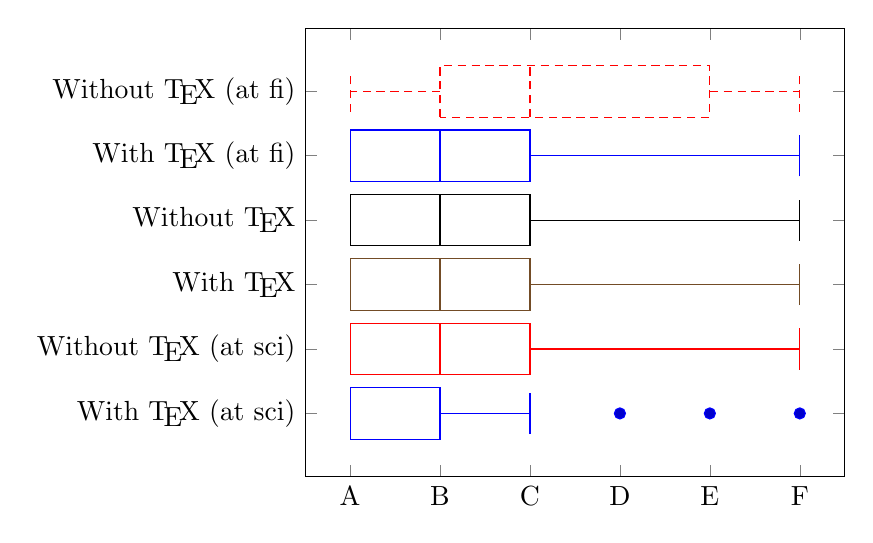
\begin{tikzpicture}
      \begin{axis}
        [
          ytick={1,2,3,4,5,6},
          xticklabels={,,A,B,C,D,E,F},
          yticklabels={With \TeX{} (at \acrshort{sci}),
                       Without \TeX{} (at \acrshort{sci}),
                       With \TeX{},
                       Without \TeX{},
                       With \TeX{} (at \acrshort{fi}),
                       Without \TeX{} (at \acrshort{fi})},
        ]
        \addplot+[
          boxplot prepared={
            lower quartile=1,
            median=1,
            upper quartile=2,
            upper whisker=3,
            lower whisker=1,
            % average=1.9148387097
          },
        ] table[row sep=\\,y index=0] {
          data\\ 4\\ 5\\ 6\\
        };
        \addplot+[
          boxplot prepared={
            lower quartile=1,
            median=2,
            upper quartile=3,
            upper whisker=6,
            lower whisker=1,
            % average=2.0201768307
          },
        ] table[row sep=\\,y index=0] {
          data\\
        };
        \addplot+[
          boxplot prepared={
            lower whisker=1,
            lower quartile=1,
            median=2,
            upper quartile=3,
            upper whisker=6,
            % average=2.2110091743
          },
        ] table[row sep=\\,y index=0] {
          data\\
        };
        \addplot+[
          boxplot prepared={
            lower whisker=1,
            lower quartile=1,
            median=2,
            upper quartile=3,
            upper whisker=6,
            % average=2.3971979233
          },
        ] table[row sep=\\,y index=0] {
          data\\
        };
        \addplot+[
          boxplot prepared={
            lower whisker=1,
            lower quartile=1,
            median=2,
            upper quartile=3,
            upper whisker=6,
            % average=2.3565375303
          },
        ] table[row sep=\\,y index=0] {
          data\\
        };
        \addplot+[
          boxplot prepared={
            lower whisker=1,
            lower quartile=2,
            median=3,
            upper quartile=5,
            upper whisker=6,
            % average=3.1209262436
          },
        ] table[row sep=\\,y index=0] {
          data\\
        };
      \end{axis}
    \end{tikzpicture}
    \caption{A box plot of the grades of theses written and
      defended during 2010--2015 at \acrshort{fi}, \acrshort{sci}
      and all the faculties of \acrshort{mu} with and without
      \gls{tex}}
    \label{fig:statistics-grades}
  \end{figure}

  Suppose the null \gls{hypothesis} $h_1$ that the grades awarded
  to theses written using and not using \gls{tex}, respectively,
  have the same distribution on the significance level
  $\alpha=0.05$. The one-tailed Pearson's $\chi^2$ test
  \cite{Pearson00} of the goodness of fit was applied to the
  observations of awarded grades that made up more than one percent
  of the sample data (grades A, B, C, D, E and F, see Table
  \ref{table:statistics-contingency}).
  Since \begin{equation}
    \sum_{\text{A},\text{B},\ldots,\text{F}}
    (\text{E}-\text{O})^2/\text{E}=104.623\gg11.07=
    \chi_{1-\alpha}^2(5)
  \end{equation} the author refused the null hypothesis $h_1$
  and concluded that the grades are indeed differently
  distributed on the significance level $\alpha$.

  Having shown that the distribution of grades awarded to theses
  written using and not using \gls{tex} is different, the author
  proceeded to inspect, if this holds for individual grades.
  Suppose the null \gls{hypothesis} $h_\text{A}$ that the
  distribution of grade A being awarded to theses written using
  \gls{tex} is equivalent to the distribution of grade A being
  awarded to theses not written using \gls{tex}. The two-tailed
  Mann-Whitney U test~\cite{mann47,manntut} was applied to the
  observations of grade A being and not being awarded to theses
  written using and not using \gls{tex}: \begin{align}
    \tag{Without \gls{tex} (grade A)} m_1 &= 15\,476 \\
    \tag{With \gls{tex} (grade A)}    m_2 &= 1\,181  \\
    \tag{Without \gls{tex} (total)} n_1 &= 42\,183 \\
    \tag{With \gls{tex} (total)}    n_2 &= 2\,692  \\
    U_1 &=  m_1(m_2\cdot0.5+(n_2-m_2))+
                  (n_1-m_1)((n_2-m_2)\cdot0.5) \\
      \nonumber&=52\,699\,952.5 \\
    U_2 &=  m_2(m_1\cdot0.5+(n_1-m_1))+
                  (n_2-m_2)((n_1-m_1)\cdot0.5) \\
      \nonumber&=60\,856\,683.5 \\
    U &= \min(U_1,U_2) = U_1 = 52\,699\,952.5
  \end{align} Since $n_1n_2\gg20$,
  $U\sim\text{N}\left(\frac{n_1n_2}2,
  \frac{n_1n_2(n_1+n_2+1)}{12}\right)$. After normalization to
  \begin{equation}
    \text{N}(0,1)\sim z =
    \frac{U-\frac{n_1n_2}2}{\sqrt{\frac{n_1n_2(n_1+n_2+1)}{12}}}
    \approx-\frac{4\,078\,365.5}{651\,662.46}\approx-6.258
  \end{equation} the two-tailed \gls{pval} $\beta$ was computed by
  the author as follows:\begin{align}
    & \operatorname{arg\,min}\limits_{\beta} P(\Phi^{-1}_{\beta/2}
        \leq z\leq\Phi^{-1}_{1-\beta/2})=\beta \\
    \nonumber& \iff\Phi^{-1}_{\beta/2}=-6.258 \iff\beta/2=1-
        \Phi(6.258)\iff\beta\approx 0
  \end{align}Since $\beta<\alpha$, the author refused the null
  \gls{hypothesis} $h_\text{A}$ on the significance level $\alpha$.
  Following a similar procedure for marks B--F, the author arrived
  at the following conclusions on the significance level $\alpha$:
  \begin{itemize}
    \item Theses written using \gls{tex} had been awarded grade A
      statistically significantly more often than theses not
      written using \gls{tex}.
    \item Theses written using \gls{tex} had been awarded grades C
      and D statistically significantly less often than theses not
      written using \gls{tex}.
    \item No statistically significant difference was observed in
      the distributions of grades B, E and F being awarded to
      theses written using and not using \gls{tex}.
  \end{itemize}
  A box plot of the grades is shown in Figure
  \ref{fig:statistics-grades}.

\chapter{Review of Existing Templates}\label{sec:review}
During December 2014--January 2015, the author also assessed
several \gls{tex} templates for the typesetting of theses in order
to gather ideas for the design of the \textsf{fithesis3}
\gls{docclass} (see Chapter~\ref{sec:des&impl}). Initially, the
author is going to focus on templates used at Czech technical
universities. At the end of the section, select generic templates
will also be considered.

  \section{Charles University and Czech Technical~University}
  \subsection{\inx{\textsf{CUStyle}} and \inx{\textsf{CTUStyle}}}
  \label{sec:ctu&custyle}
  The first of the reviewed thesis typesetting templates were the
  \textsf{CUStyle} \cite{custyle} and \textsf{CTUStyle}
  \cite{ctustyle} \glspl{texpackage} from RNDr.\ Petr Olšák,
  which were designed to be used at \gls{cuni} and at \gls{fel},
  respectively. The sole dependencies of these templates are the
  \gls{csplain} and \gls{opmac} packages.

  The templates are closely tied with the visual styles of the
  universities, which is mainly achieved through color-coding.
  Aside from black-and-white text, the \textsf{CTUStyle}
  \gls{texpackage} typesets various typographic elements in the
  \clrpicker{pantone300} Pantone 300 color, which makes for a
  visually pleasing combination. The \textsf{CUStyle}
  \gls{texpackage} uses the combination of black, gray and
  \clrpicker{cured} Pantone 1797 color to a similar end. 

  Unlike with \textsf{fithesis2}, documents typeset with the
  \textsf{CTUStyle} and \textsf{CUStyle} templates are double-sided
  by default. The \gls{textwidth} of \textsf{CTUStyle}
  \eqref{eq:ctustyle-textwidth} and \textsf{CUStyle}
  \eqref{eq:custyle-textwidth}
  \begin{align}
    \label{eq:ctustyle-textwidth} 210\text{\,mm}\text{ (A4 width) }
      &- 2\cdot32\text{\,mm} \text{ \cite[line~249]{ctustyleCode} }
      &= 146\text{\,mm} \\
    \label{eq:custyle-textwidth}  210\text{\,mm}\text{ (A4 width) }
      &- 2\cdot31\text{\,mm} \text{ \cite[line~229]{custyleCode} }
      &= 148\text{\,mm}
  \end{align} is also much larger than that of \textsf{fithesis2}
  (127\,mm \cite[lines~989, 1017, 1045]{fithesis2Code}). The
  margins of \textsf{CTUStyle} and \textsf{CUStyle}, in conjunction
  with the chosen font family, \label{overlong-lines} allow for up
  to 100 characters per line, which is not only wearying to the eye
  of an inexperienced reader~\cite[section~2.1.2]{eletypostyle},
  but also against the recommendations of \gls{fi}
  \cite[section~3.2.3]{bpdpfi}. According to the statements of the
  author of the styles~\cite[post~25]{ctustyle-forums}, both
  decisions have likely been made in an effort to reduce the
  required storage space for the archival of physical prints of
  theses.

  \subsection{Official template of Czech Technical University}
  \label{sec:felthesis}\index{\textsf{felthesis}} The
  \textsf{felthesis} \gls{docclass} from Ing.\ Vít Zýka Ph.D.\
  provides an alternative for those \gls{fel} students, who prefer
  \gls{latex} over \gls{csplain} used by the
  \inx{\textsf{CTUStyle}} \gls{texpackage}. Much like
  \textsf{fithesis1} and \textsf{fithesis2}, \textsf{felthesis}
  loads the KOMA-Script \textsf{scrreprt} \gls{docclass}, redefines
  some of its commands and \glspl{env}, loads additional packages
  and defines additional thesis sectioning commands. Unlike
  \textsf{fithesis1} and \textsf{fithesis2}, \textsf{felthesis}
  loads the \textsf{babel} \gls{ltxpackage}, whose main language it
  chooses based on the language of the thesis
  \cite[lines~687--691]{felthesisCode}. \textsf{Felthesis} also
  loads \gls{biblatex}~\cite[line~722]{felthesisCode},
  automatically generates index~\cite[line~763]{felthesisCode} and
  stamps the title, author, subject, and keywords into the header
  of the resulting \gls{pdf}
  file~\cite[lines~959--971]{felthesisCode}\label{pdf-stamping}.
  Alongside the \gls{ltxpackage}, both a technical
  \cite{felthesisCode} and a user documentation \cite{felthesis} is
  distributed. The \textsf{felthesis} \gls{docclass} can be
  downloaded from \cite{felthesisPkg}.

  \subsection{Official template of Charles University}
  Along with Petr Olšák's \textsf{CUStyle}, \gls{cuni} also
  provides an official \gls{latex} template for the typesetting of
  theses. Rather than defining a new
  \gls{docclass}, the archive contains a \gls{makefile} and a
  skeleton \gls{latex} document using the base \textsf{report}
  \gls{docclass} for both Czech and English theses. The students
  are expected to modify the said document to suit their
  requirements. The template uses \gls{cslatex} rather than the
  babel \gls{ltxpackage}, which means that \gls{csfonts} rather
  than the superior \gls{lmfonts}~\cite{cslatexvsbabel} are used
  by default. Likewise problematic is the implicit \gls{textwidth}
  of 145\,mm \cite[line~7]{cunicode}, which, in conjunction with
  the usage of \gls{csfonts} at 12\,pt, allows for up to 100
  characters per line. This is problematic for reasons mentioned in
  Subsection \ref{overlong-lines}. The template can be downloaded
  from \cite{cunisablona}.

  \section{Mendel University in Brno}\index{\texttt{dipp.sty}|(}
  \label{sec:dipp.sty}
  Despite not being an official thesis template of \gls{mendelu},
  the \texttt{dipp.sty} \gls{ltxpackage} from Doc.\ Ing.\ Dr.\ Jiří
  Rybička warrants a mention. The \gls{ltxpackage} depends on the
  extended macro set of the \Hologo{XeTeX}
  \glslink{texeng}{typesetting engine} and is intended to be used
  with the base \textsf{article} \gls{docclass}. Although the
  article class was not designed with European typography in mind,
  the \texttt{dipp.sty} \gls{ltxpackage} redefines much of the
  geometry. The implicit \gls{textwidth} of the \gls{ltxpackage} is
  150\,mm \cite[line~26]{dipp.sty}, which allows for up to 90
  characters per line. This is problematic for reasons mentioned in
  Subsection \ref{overlong-lines}.

  Noteworthy is the rich selection of additional markup, which
  is meant to ease the task of typesetting a thesis for those
  unfamiliar with \gls{latex}. To this end, the \gls{ltxpackage}
  defines thesis sectioning commands, macros and wrapper
  \glspl{env} for the inclusion of bibliography, tables or figures
  and discretionary macros specific to Czech typography such as
  \cs{az} for the typesetting of ranges and \cs{spoj} for
  hyphenation \cite{dippman}. The \texttt{dipp.sty} \gls{ltxpackage}
  can be downloaded from \cite{dipp.sty}.\index{\texttt{dipp.sty}|)}

  \section{Brno University of Technology}
  \index{\texttt{thesis.sty}|(}
  The official thesis typesetting template of \gls{vut} is the
  \texttt{thesis.sty} \gls{ltxpackage}. Unlike
  \texttt{\hyperref[sec:dipp.sty]{\tt dipp.sty}},
  \texttt{thesis.sty} is meant to be used with the base
  \textsf{report} \gls{docclass}. All \glspl{ltxpackage} required
  by the \gls{ltxpackage} are documented within the
  \gls{ltxpackage} documentation \cite[p.~9]{thesis.sty-doc}. The
  implicit \gls{textwidth} of the \gls{ltxpackage} is 150\,mm
  \cite[p.~2]{thesis.sty-doc}, which, in conjunction with the usage
  of \gls{csfonts} at 12\,pt, allows for up to 90 characters per
  line. This is problematic for reasons mentioned in Subsection
  \ref{overlong-lines}.

  The \texttt{thesis.sty} \gls{ltxpackage} also adds
  additional markup. This includes wrapper commands such as
  \cs{novazkratka}, \cs{zk}, \cs{zkratka} and \cs{zkratkatext} for
  the typesetting of acronyms, the \cs{seznamzkratek} and
  \cs{literatura} \glspl{env} for acronyms and bibliography,
  respectively, and various math mode macros (see
  \cite[p.~6--9]{thesis.sty-doc}). Like
  \hyperref[sec:felthesis]{\textsf{felthesis}},
  \texttt{thesis.sty} is also able to stamp thesis metadata into
  the \gls{pdf} header. The \texttt{thesis.sty} \gls{ltxpackage}
  can be downloaded from \cite{thesis.sty}.
  \index{\texttt{thesis.sty}|)}

  \section{Technical University of Liberec}
  \index{\textsf{tul}|(}\index{\textsf{tulthesis}|(} Unlike the
  preceding typesetting templates, \textsf{tulthesis} from Doc.\
  RNDr.\ Pavel Satrapa,\ Ph.D.\ is not a standalone \gls{docclass},
  but rather a part of the \textsf{tul} \gls{ltxpackage}, which is
  the official \gls{ltxpackage} used for the typesetting of
  documents on \gls{tul}. \textsf{Tulthesis} uses the base
  \textsf{report} \gls{docclass} \cite[section~1]{tulthesis-man},
  supports modern \glspl{texeng} such as \Hologo{XeTeX}, and
  \Hologo{LuaTeX}, and is quite visually distinctive. An interesting
  bit of trivia is the fact that the template inspired
  \cite[post~21]{ctustyle-forums} the creation of Petr Olšák's
  \nameref{sec:ctu&custyle} \glspl{texpackage}. The \textsf{tul}
  \gls{ltxpackage}, along with the tulthesis \gls{docclass}, can
  be downloaded from \cite{tul}.
  \index{\textsf{tul}|)} \index{\textsf{tulthesis}|)}

  \section{Technical University of Ostrava}\index{\textsf{diploma}|(}
  The official style for the typesetting of documents at \gls{vsb}
  is the \textsf{diploma} \gls{docclass} by Jiří Dvorský. Like Jiří
  Rybička's \hyperref[sec:dipp.sty]{\tt dipp.sty}, \textsf{diploma}
  uses the base \textsf{article} \gls{docclass}, modifies its
  geometry and adds thesis sectioning commands and additional
  macros for the users' convenience \cite{diploma}. The output
  documents are one-sided by default and the font size of 11\,pt is
  too small for the \gls{textwidth} of \begin{equation}
    \begin{split}
      210\,\text{mm} \text{ (A4 width) }
        &- 28\,\text{mm} \text{ (left margin) }  \\
        &- 32\,\text{mm} \text{ (right margin) } = 150\,\text{mm}
    \end{split}
  \end{equation} as defined in
  \cite[lines~111,~123]{diplomaSource}, resulting in overlong lines
  as discussed earlier (see Subsection \ref{overlong-lines}).

  The additional macros range from mathematical \glspl{env}
  \cite[section~3.5]{diploma} and commands and \glspl{env} for the
  typesetting of code with syntax highlighting
  \cite[section~3.6]{diploma} through commands for the insertion of
  graphics \cite[section~3.7]{diploma}. \index{\textsf{diploma}|)}

  \section{Silesian University in Opava}
  At the time of the reasearch, there was no official or unofficial
  \gls{gls-docclass} or \gls{ltxpackage} of \gls{slu} available on
  the Internet. There is a mention \cite{vavreckova} of the works
  on a \gls{docclass} at the webpage of RNDr.\ Šárka Vavřečková,
  Ph.D.\ who teaches typography at \acrlong{fpf}. There is also a
  bachelor's thesis~\cite{hanzal09} written by Michal Hanzal from
  \gls{opf} who describes the process of creating a
  \gls{gls-docclass} for what is supposed to be the official thesis
  typesetting template at \gls{opf}. There is, however, no mention
  of the style at the website of the faculty \cite{opftemplates},
  although the linked Dean's directives were written with
  \gls{latex} in mind. \emph{Enshrouded in mystery} is, the author
  opines, the only accurate way to describe the state of affairs.

  \section{Palacký University Olomouc}\label{sec:upol}
  There are three independent \gls{latex} thesis typesetting
  templates available at \acrlong{upolsci} provided by the
  departments of Experimental Physics, Informatics and Mathematical
  Analysis and Applications, respectively.

  The template used at the Department of Experimental Physics is
  just an example \gls{latex} document using the base
  \textsf{article} class, which the students are expected to edit
  according to their needs. The template is supposed to be typeset
  using the \glslink{cslatex}{\pdfCSLaTeX{}} \gls{texeng} meaning
  that \gls{csfonts} instead of the superior \gls{lmfonts} are
  used.  Along with the thesis template, a \gls{beamer} template
  for thesis defense presentations is also distributed.  Both
  templates can be downloaded at \cite{upol-exfyz-template}.

  \index{\textsf{KIdiplom}|(} The template used at the Department
  of Informatics is \textsf{KIdiplom} from Jan Outrata and Martin
  Rotter and it is a combination of a \gls{docclass}, which is
  built on the base \textsf{article} \gls{docclass} and is meant
  for the typesetting of theses, and a \gls{ltxpackage}, which was
  designed as a general template for the typesetting of documents
  in the visual style of the Department of Informatics. Amongst
  the vices of the template are the disabled double-sided
  typesetting \cite[lines~69--72]{upol-inf-templateSource} and the
  \gls{textwidth} of\begin{equation}
    426\text{\,pt}\text{ (\texttt{a4paper} \gls{textwidth}) }
    \cdot1{,}05\text{ \cite[line~81]{upol-inf-templateSource} }
    \approx157,23\text{\,mm}
  \end{equation} which, in conjunction with the 12\,pt
  \gls{lmfonts} is, the author opines, too generous
  \cite[lines~74--82]{upol-inf-templateSource} and causes
  overlong lines (see Subsection \ref{overlong-lines}). The
  template implicitly loads \gls{biblatex} and \glspl{ltxpackage}
  for the typesetting of glossaries and index. The added
  convenience macros comprise thesis sectioning commands and
  \glspl{env} for the typesetting of mathematical definitions,
  theorems or proofs as well as code snippets. Along with the
  thesis template, \gls{latex} templates for the typesetting of
  thesis reader's reports and \gls{biblatex}
  ISO\hyph{}690~\cite{iso690-1,iso690-2} citation styles\pending{}
  are distributed. The templates can be downloaded at
  \cite{upol-inf-template}.\index{\textsf{KIdiplom}|)}

  \index{\texttt{maam-dipl.sty}|(}The template used at the
  Department of Mathematical Analysis and Applications is the
  \texttt{maam-dipl.sty} \gls{ltxpackage}, which only defines basic
  thesis sectioning commands and is meant to be used with the base
  \textsf{article} \gls{docclass}. The template can be downloaded
  at \cite{upol-maam-template}\index{\texttt{maam-dipl.sty}|)}.

  \section{Masaryk University in Brno}\label{sec:muni-styles}
  Aside from \gls{fi}, the only other faculty of \gls{mu} to offer
  a thesis typesetting template in \gls{tex} was \gls{sci}. This
  is in line with the statistics of usage of \gls{tex}, which are
  by and large dominated by \gls{fi} and \gls{sci} (see Section
  \ref{sec:statistics}). The template used at \gls{sci} is the
  \texttt{sci.muni.thesis.sty}\index{\texttt{sci.muni.thesis.sty}}
  \gls{ltxpackage}, which is intended to be used with the base
  \textsf{book} \gls{docclass}. The output documents are one-sided
  by default and the font size of 12\,pt is too small for the
  \gls{textwidth} of \begin{equation}\begin{split}
    210\,\text{mm} \text{ (A4 width) }
    &- 34\,\text{mm} \text{ (left margin) }  \\
    &- 25\,\text{mm} \text{ (right margin) } =
    151\,\text{mm}\end{split}\end{equation} as defined in
  \cite[line~109]{scimuni-thesisSource}, resulting in overlong
  lines as discussed earlier (see Subsection \ref{overlong-lines}).

  \section{Generic templates}
  Amongst the noteworthy generic thesis typesetting templates the
  author had the opportunity to encounter was the
  \textsf{classicthesis} \index{\textsf{classicthesis}}
  \gls{ltxpackage}, which heavily modifies the \textsf{scrreprt}
  KOMA-Script \gls{docclass} in an endeavor to replicate the design
  of Bringhurst's \emph{The Elements of Typographic Style}
  \cite{eletypostyle}. The author notes that the
  \textsf{classicthesis} \gls{ltxpackage} is one of the few that
  manage to avoid overlong lines (see Subsection
  \ref{overlong-lines}). The \gls{ltxpackage} can be downloaded at%
  ~\cite{classicthesis}.

  Another generic thesis typesetting template, which the author
  found refreshing, was the
  \textsf{graduate-thesis}\index{\textsf{graduate-thesis}}
  \gls{docclass}, which is based on the base \textsf{book}
  \gls{docclass} and which, like
  \hyperref[sec:ctu&custyle]{\textsf{CTUStyle}%
  \index{\textsf{CTUStyle}}}, uses a visually pleasing combination
  of black and blue. Like most of the reviewed templates,
  \textsf{graduate-thesis}, too, suffers from overlong lines (see
  Subsection \ref{overlong-lines}). The \gls{ltxpackage} can be
  downloaded at \cite{graduate-thesis}.

  % CTAN: http://www.ctan.org/topic/dissertation
  % Kumar07, https://tug.org/pracjourn/2007-4/

\chapter{Design and Implementation}\label{sec:des&impl}
Following the analysis of the usage of \gls{tex} at \gls{mu} (see
Chapter \ref{sec:texusage}) and the review of existing thesis
typesetting templates (see Chapter \ref{sec:review}) conducted
during December 2014--January 2015, the author developed a new
\textsf{fithesis3} \gls{docclass} during January--May 2015. In this
chapter, the author is going to describe the main goals of the
\gls{docclass} along with its design and implementation.

  \section{Goals}
  The \textsf{fithesis2} document class included the logos of all
  faculties of \gls{mu}, which in theory enabled its usage across
  the faculties of \gls{mu}. In practice, however, each faculty of
  \gls{mu} had a vastly different rules regarding the structure and
  the formatting of theses. These differences had to be resolved by
  the end users, which decreased the usefulness of the class. One
  of the main goals of \textsf{fithesis3} was therefore the
  addition of a more comprehensive support for the various
  faculties of \gls{mu}.

  With the advent of the digital age, the importance of printed
  works has diminished in favour of electronic documents. Another
  main goal of \textsf{fithesis3} was therefore better utilization
  of the \gls{pdf} format capabilities, as demonstrated by the
  \index{\textsf{felthesis}}%
  \hyperref[sec:felthesis]{\textsf{felthesis}}
  \gls{docclass} (see Section \ref{sec:felthesis}). Other goals
  included the addition of support for modern \glspl{texeng} other
  than \TeX{} and \hologo{pdfLaTeX} and the addition of support for
  color printing.

  \section{Design}
  The \textsf{fithesis1} and \textsf{fithesis2} \glspl{docclass}
  had the following responsibilities: \begin{enumerate}
    \item The management of Czech, Slovak and English locale
      strings
    \item The definition of the document style
    \item The processing of the class options and thesis metadata
  \end{enumerate} These responsibilities had been hard-wired into
  the \glspl{docclass} with little thought given to extensibility.  
  With the addition of support for faculties other than \gls{fi},
  it was necessary to enable easy addition of new languages such as
  French \cite{Zeman14} or Russian \cite{Kupcevic14}. To enable the
  automatic typesetting of the mandatory parts of theses in
  compliance with the requirements of the faculties of \gls{mu},
  new metadata fields also had to be added to the class and the
  document style had to respond to the faculty at which the thesis
  was going to be written and defended.
  
  For these reasons, the author had decided to decompose the class
  into the following parts: \begin{enumerate}
    \item\emph{Locale files} that encapsulate locale strings
    \item\emph{Style files} that define the look and layout of the
      document
    \item\emph{The \gls{docclass} file} that processes the user
      input and loads the according locale and style files
  \end{enumerate} When a user specified the \gls{docclass} in the
  preamble of the document, only the \gls{docclass} file would get
  loaded. The user would then input the metadata of their thesis,
  which would be processed by the \gls{docclass}. If no metadata
  were input, placeholder values would be used instead. At the end
  of the preamble, the metadata would be written to the header of
  the output document, the corresponding locale and style files
  would be loaded and the mandatory parts specified by the style
  file would be appended to the document.

  The compatibility with various \glspl{texeng} would be ensured by
  the style files, which would detect the engine used and behave
  accordingly. The support for color printing would likewise be
  added at the style file level.

  \section{Implementation}
  The directory structure of \textsf{fithesis3} is shown in Figure
  \ref{fig:dirs}. The \texttt{locale/} and \texttt{style/}
  directories contain the locale and style files and the
  \texttt{logo/} directory contains the university
  and faculty logos in \gls{pdf} and \gls{eps} formats. The
  \texttt{fithesis3.cls} file represents the \textsf{fithesis3}
  \gls{docclass}.

  \begin{figure}
    \centering
    \parbox{0.5\textwidth}{\dirtree{%
      .1 fithesis3/.
        .2 locale/.
        .2 style/.
        .2 logo/.
        .2 fithesis3.cls.
    }}
    \caption{The directory structure of \textsf{fithesis3}}
    \label{fig:dirs}
  \end{figure}
  
  \subsection{Locale files}
  The structure of the \texttt{locale/} directory is shown in in
  Figure \ref{fig:dirs-locale}. The locale files of a given
  locale for a given faculty of a given university are named
  \texttt{\textit{locale}.def} and are
  loaded from the least to the most specific one starting at the
  root of the \texttt{locale/} directory and ending up in the
  \texttt{\textit{university}/\textit{faculty}/}
  subdirectory. The motivation for this
  scheme was code reuse. If each of $m$ faculties at $n$
  universities used the same $k$ strings, then $(\begin{smallmatrix}
  kmn\\2\end{smallmatrix})$ pairs of strings would need to be kept
  mutually consistent. An inheritance scheme largely eliminated
  this problem by allowing the creation of one copy of the $k$
  shared strings, which is shared by the subsequently loaded $mn$
  locale files.

  For documentation and maintenance purposes, each locale consists
  of only one \texttt{\textit{locale}.dtx} \gls{dtx} file stored
  within the \texttt{locale/} directory. This file is decomposed
  into individual files using the \texttt{\textit{locale}.ins}
  \gls{ins} file and the \gls{makefile} stored within the
  \texttt{locale} directory.

  \begin{figure}
    \centering
    \parbox{0.5\textwidth}{\dirtree{%
      .1 locale/.
        .2 \textit{locale}.def.
        .2 \textit{university}/.
          .3 \textit{locale}.def.
          .3 \textit{faculty}/.
            .4 \textit{locale}.def.
    }}
    \caption{The directory structure of the locale files of
      \textsf{fithesis3}}
    \label{fig:dirs-locale}
  \end{figure}
  
  \subsection{Style files}\label{sec:dev-styles}
  The structure of the \texttt{style/} directory is shown in Figure
  \ref{fig:dirs-style}. The style files for a given faculty of a
  given university are named
  \texttt{fithesis3\hyph{}\textit{faculty}.sty} and
  are stored within the \texttt{\textit{university}/}
  subdirectory. Common behavior is inherited from the
  \texttt{fithesis3\hyph{}base.sty} style files,
  which, much like locale files, are loaded from the least to the
  most specific one starting at the root of the \texttt{style/}
  directory and ending up in the
  \texttt{\textit{university}/} subdirectory. The
  \texttt{fithesis3-} filename prefix serves to prevent naming
  collisions. Since the style files are ordinary \LaTeX{} packages
  and the \gls{tds} is flat, naming the style files only
  \texttt{\textit{faculty}.sty} would run the risk of clashing with
  a similarly named \gls{ltxpackage}.

  The majority of the style files of \gls{mu} were developed in
  accordance with Dean's directives or formal requirements
  published at the website of the faculties \cite{ffdirective,
  peddirective,scidirective,lawdirective,fidirective,fspsdirective}.
  The exceptions were \gls{fss} and \gls{lf}. At \gls{fss}, there
  was a multitude of conflicting recommendations by its various
  departments with no unifying set of requirements. A skeleton
  style file was created, which the user can alter
  in accordance with the requirements of the given department. At
  \gls{lf}, only the department of optometrics specified any
  formal requirements~\cite{meddirective}. The style file of
  \gls{lf} was therefore prepared in accordance with these
  requirements. The style file of \gls{sci} also warrants a
  mention, since it was deliberately designed to resemble the
  thesis typesetting template of \gls{sci} (see Section
  \ref{sec:muni-styles}) in order to facilitate the adoption of
  \textsf{fithesis3} at \gls{sci}.
  
  The compatibility of the style files of \gls{mu} with the
  \Hologo{XeTeX} and \Hologo{LuaTeX} \glspl{texeng} is implemented
  by the \texttt{fithesis3-base.sty} style file stored within the
  \texttt{mu/} directory, which loads \gls{texeng}-specific
  packages based on the \gls{texeng} used. Drawing inspiration
  from Petr Olšák's \hyperref[sec:ctu&custyle]{\textsf{CTUStyle}
  \index{\textsf{CTUStyle}} and
  \textsf{CUStyle}\index{\textsf{CUStyle}} \glspl{texpackage}}
  (see Section \ref{sec:ctu&custyle}), the addition of support for
  colorful typesetting was added to the style files of \gls{mu}
  spanning links, tables and the university and faculty logos.

  For documentation and maintenance purposes, the style file for
  each faculty of a given university consists of one
  \texttt{\textit{faculty}.dtx} \gls{dtx} file stored within the
  \texttt{\textit{university}/} subdirectory. This file is
  converted into the \texttt{fithesis3-\textit{faculty}.sty} file
  using the \texttt{\textit{faculty}.ins} \gls{ins} file and the
  \gls{makefile} stored within the \texttt{locale/} directory.
  
  \begin{figure}
    \centering
    \parbox{0.5\textwidth}{\dirtree{%
      .1 style/.
        .2 fithesis3-base.sty.
        .2 \textit{university}/.
          .3 fithesis3-base.sty.
          .3 fithesis3-\textit{faculty}.sty.
    }}
    \caption{The directory structure of the style files of
      \textsf{fithesis3}}
    \label{fig:dirs-style}
  \end{figure}
  
  \subsection{Logo files}
  The structure of the \texttt{logo/} directory is shown in Figure
  \ref{fig:dirs-logo}. The university logo of a given
  university is stored in the \texttt{base.pdf} \gls{pdf} and
  \texttt{base.eps} \gls{eps} files within the
  \texttt{\textit{university}/} subdirectory. The faculty logo for
  a given faculty of a given university is stored in the
  \texttt{\textit{faculty}.pdf} \gls{pdf} and
  \texttt{\textit{faculty}.eps} \gls{eps} files within
  the \texttt{\textit{university}/} subdirectory. The
  \texttt{\textit{university}/color/} subdirectory is required by
  the style files of \gls{mu} when color printing is enabled and
  contains the color versions of logos in an identical directory
  structure.

  \begin{figure}
    \centering
    \parbox{0.5\textwidth}{\dirtree{%
      .1 logo/.
        .2 \textit{university}/.
          .3 base.eps.
          .3 base.pdf.
          .3 \textit{faculty}.eps.
          .3 \textit{faculty}.pdf.
          .3 color/.
            .4 base.eps.
            .4 base.pdf.
            .4 \textit{faculty}.eps.
            .4 \textit{faculty}.pdf.
    }}
    \caption{The directory structure of the style files of
      \textsf{fithesis3}}
    \label{fig:dirs-logo}
  \end{figure}
  
  The monochrome and color versions of the logos in \gls{eps}
  format were downloaded from the website of \gls{mu} \cite{muvis}
  and subsequently converted to \gls{pdf} using the
  \textsf{epstopdf} utility. The only exception was the
  logo of \gls{fi}, which was instead taken from the bachelor's
  thesis of Mgr.\ Matúš Kominka \cite{Kominka08}. Figure
  \ref{fig:logo} contrasts the vector logo with the original
  \gls{metafont} logo designed by \thesis{advisor}\ and
  implemented by the founding Dean of \gls{fi}, Prof.\ Jiří
  Zlatuška~\cite{filogo}.

  For maintenance purposes, the logo files consist of only the
  \gls{eps} files. The \gls{eps} files can be converted into
  \gls{pdf} files using the \glspl{makefile} stored in the
  \texttt{\textit{university}/} and 
  \texttt{\textit{university}/color/}
  subdirectories.

  \begin{figure}
    \includegraphics[clip,trim=4.25cm 19.2cm 4.25cm 5.8cm]%
      {misc/metaveps.pdf}
    \caption{A comparison of the \gls{metafont} and the vector
      logo of \acrshort{fi} at 40\,mm}
    \label{fig:logo}
  \end{figure}

  \subsection{The class file}
  With the majority of the \textsf{fithesis2} code being reduced to
  layout definitions in the \texttt{fithesis3-base.sty} style file
  and the \texttt{fithesis3-10}, \texttt{11} and \texttt{12.clo}
  class options files, the \textsf{fithesis3} \gls{docclass} was
  written from scratch. Although most of the class file concerns
  dry processing of the input metadata, there are some parts that
  warrant a mention. Specifically, the support for automatic locale
  detection detection was added, drawing inspiration from the
  \hyperref[sec:felthesis]{\textsf{felthesis}} \gls{docclass} (see
  Section \ref{sec:felthesis}). \textsf{Fithesis3} automatically
  detects the main language of either the \textsf{babel} or the
  \textsf{polyglossia} package and sets it as the locale, when the
  locale is unspecified by the user.

  In order to be future-proof for the modern \gls{tex} engines, the
  class mandates the use of the UTF-8 \gls{charenc}. This is also
  in line with the belief of the author that the production of new
  documents in \glspl{charenc} other than UTF-8 hinders
  accessibility, has no grounds and should be avoided.

  For documentation and maintenance purposes, the
  \textsf{fithesis3} \gls{docclass} file consists of only one
  \texttt{fithesis.dtx} \gls{dtx} file stored within the root
  directory of the class. This file is converted into the
  \texttt{fithesis3.cls} file using the
  \texttt{\textit{locale}.ins} \gls{ins} file and the
  \gls{makefile} stored within the root directory. The \texttt{all}
  target of this \gls{makefile} can be used to build all the locale
  and style files as well as the \texttt{fithesis3.cls} file. The
  \texttt{complete} target of this \gls{makefile} typesets the
  technical documentation of the \gls{docclass} \cite{novotny15}
  into the \texttt{fithesis.pdf} file stored within the root
  directory. The target also typesets the user documentation of the
  \gls{docclass} into the \texttt{\textit{faculty}.pdf} files
  stored within the \texttt{guide/\textit{university}/}
  subdirectory.

  \section{Further reading}
  To familiarize themselves with the \gls{docclass}, the reader
  is advised to consult the user documentation in appendices
  \ref{sec:figuide}--\ref{sec:fspsguide}. In case of further
  interest, the technical documentation of the \gls{docclass}
  contains a detailed description of the complete public and
  private interface of the \gls{docclass} and is available in
  Appendix \ref{sec:techdoc}. 

\chapter{Conclusion}
In the thesis, the author described the state of the \gls{latex}
thesis typesetting templates at \gls{mu} and the related software
projects prior to the author's involvement and delineated the
author's contributions to the projects.

The author then performed an analysis of the trends in the usage of
\gls{tex} at \gls{fi}, concluding that there has been a steady rise
in the use of \gls{tex} and that there has been a statistically
significant correlation between the use of \gls{tex} and the grades
being awarded to theses at \gls{mu} in the recent years. The author
then proceeded to perform a review of the typesetting styles used
at Czech universities and of generic typesetting templates. The
results of the research were accepted for publication in the \CS
TUG bulletin \cite{cstug}.

Finally, the author designed and implemented a new
\textsf{fithesis3} \gls{docclass}, which will be used for the
typesetting of theses at the faculties of \gls{mu}. Along with this
thesis, several other theses were prepared using the
\textsf{fithesis3} \gls{docclass} already this semester
\cite{kovanda15,zvolanek15,rucka15}. Being a part of the Dean's
program for the support of software development projects, the
testing of the \textsf{fithesis3} \gls{docclass} will continue
until the end of June 2015, when it will be published at online
collaboration platforms, \gls{ctan} and the website of \gls{fi}.

During July--September 2015, the user guide will be expanded to its
full length reflecting the user feedback submitted to the
discussion forum \cite{fithesisForum}. An author's cookbook
summarizing the formal requirements for theses will also be created
and, drawing inspiration from the Department of Experimental
Physics and the Department of Informatics at \gls{upol} (see
Section \ref{sec:upol}), so will a \gls{beamer} template for thesis
defense presentations and a template for the typesetting of
reader's reports by thesis advisors and opponents. During the
following semesters, the \textsf{fithesis3} \gls{docclass} will
become a part of the curriculum of the \emph{PB029 -- Electronic
Document Preparation} subject taught at \gls{fi}.

\begin{appendices}
\chapter{List of Electronic Attachments}\label{sec:el-att}
Along with the thesis, the author also submitted the following
files: \begin{itemize}
  \item\texttt{fithesis.zip} -- The current release of the
    \textsf{fithesis3} \gls{docclass} along with its source. This
    material is subject to the \LaTeX\ Project Public License.
  \item\texttt{survey.csv} -- A \gls{csv} file containing the
    results of the questionnaire regarding the usage of \gls{tex}
    for the writing of theses at \gls{mu}, as detailed in Section
    \ref{sec:survey}
  \item\texttt{statistics.zip} -- A \gls{zip} archive containing
    the statistical data of theses written and defended during
    2010--2015 at \gls{mu}, as detailed in Section
    \ref{sec:statistics}
  \item\texttt{thesis.zip} -- A \gls{zip} archive containing the
    full \gls{latex} source of this thesis and related resources
\end{itemize}

Appendices \ref{sec:figuide}--\ref{sec:fspsguide} contain the user
documentation of the template for the various faculties of \gls{mu}
and Appendix \ref{sec:techdoc} contains the full technical
documentation of the template. The author trusts that the kind
reader will excuse some typographical deficiencies within the
technical documentation.

\fakechapter{A \textsf{fithesis3} user guide for the Faculty of
  Informatics}\label{sec:figuide}
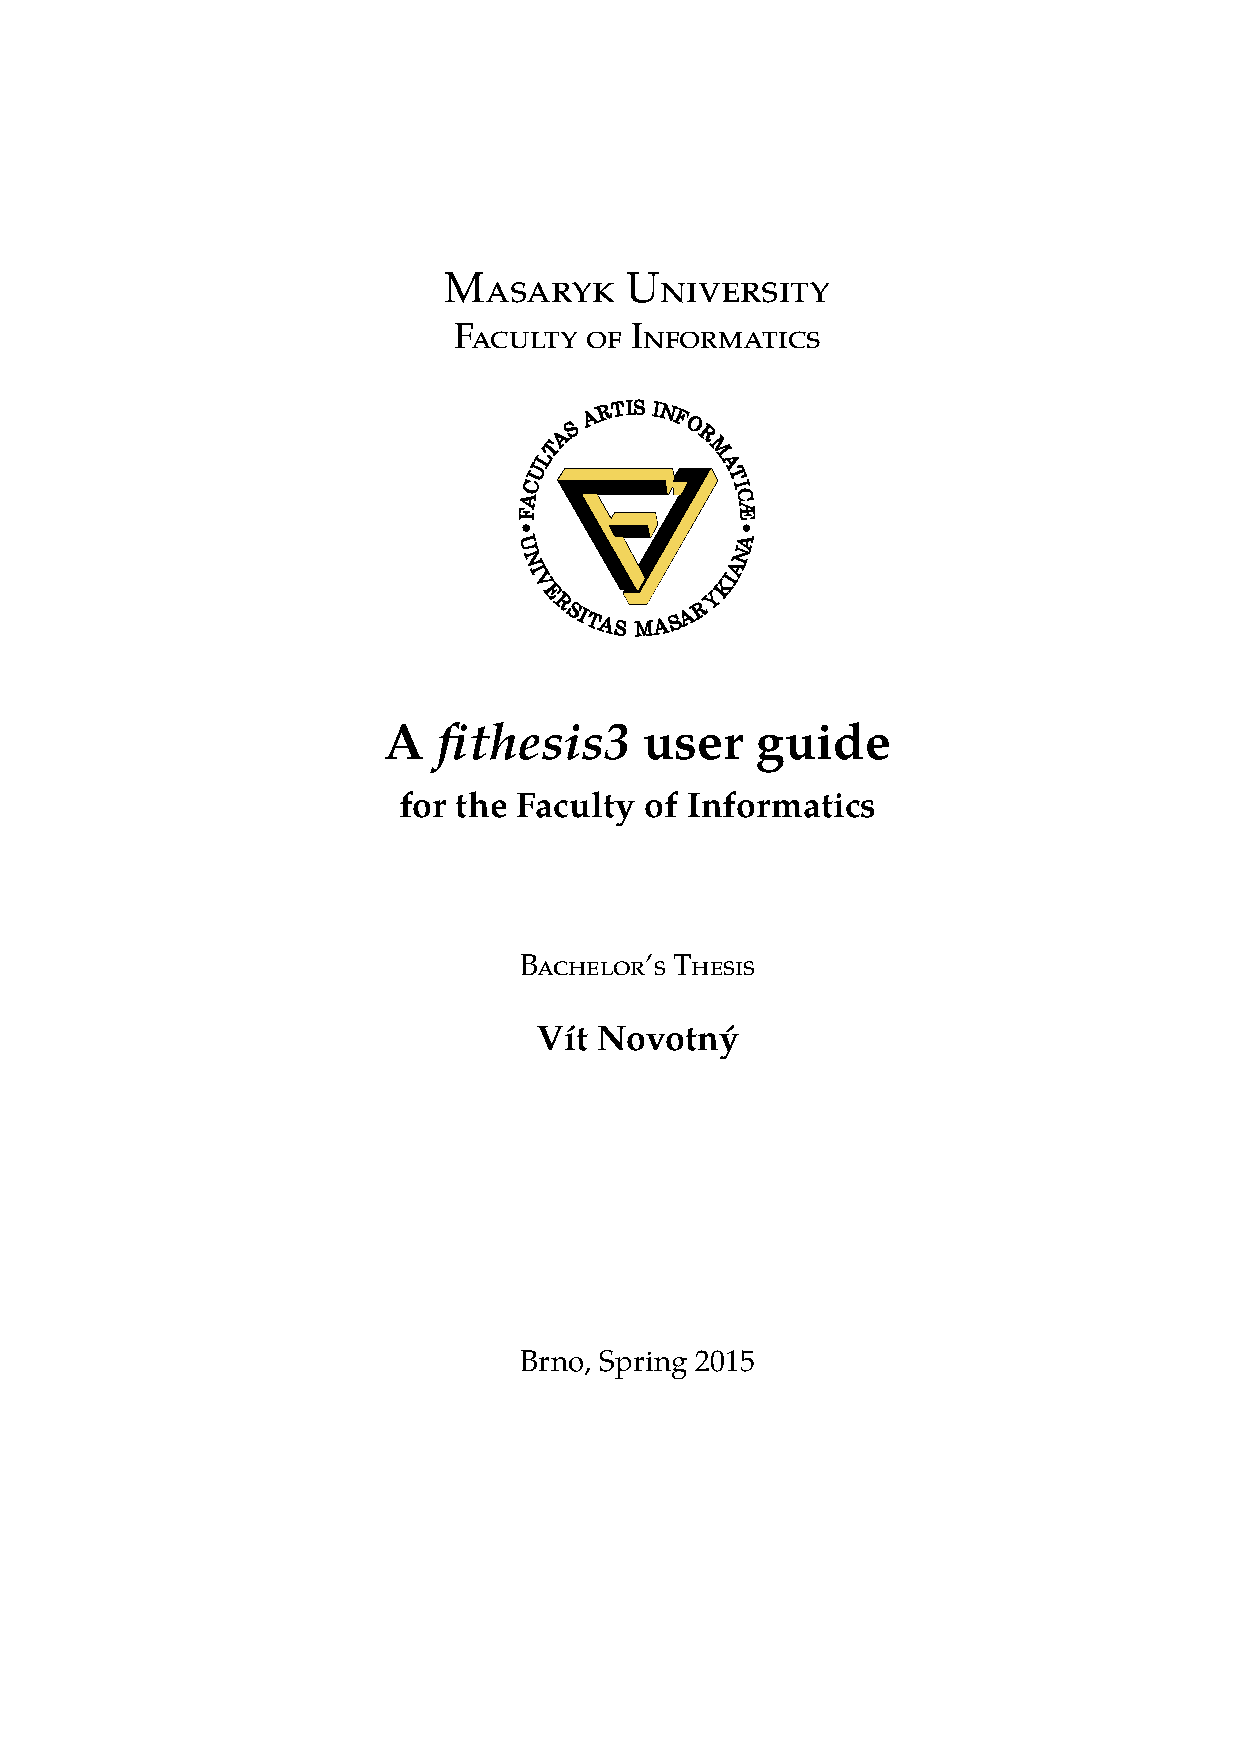
\includepdf[pages=-]{misc/fi.pdf}

\fakechapter{A \textsf{fithesis3} user guide for the Faculty of
  Science}
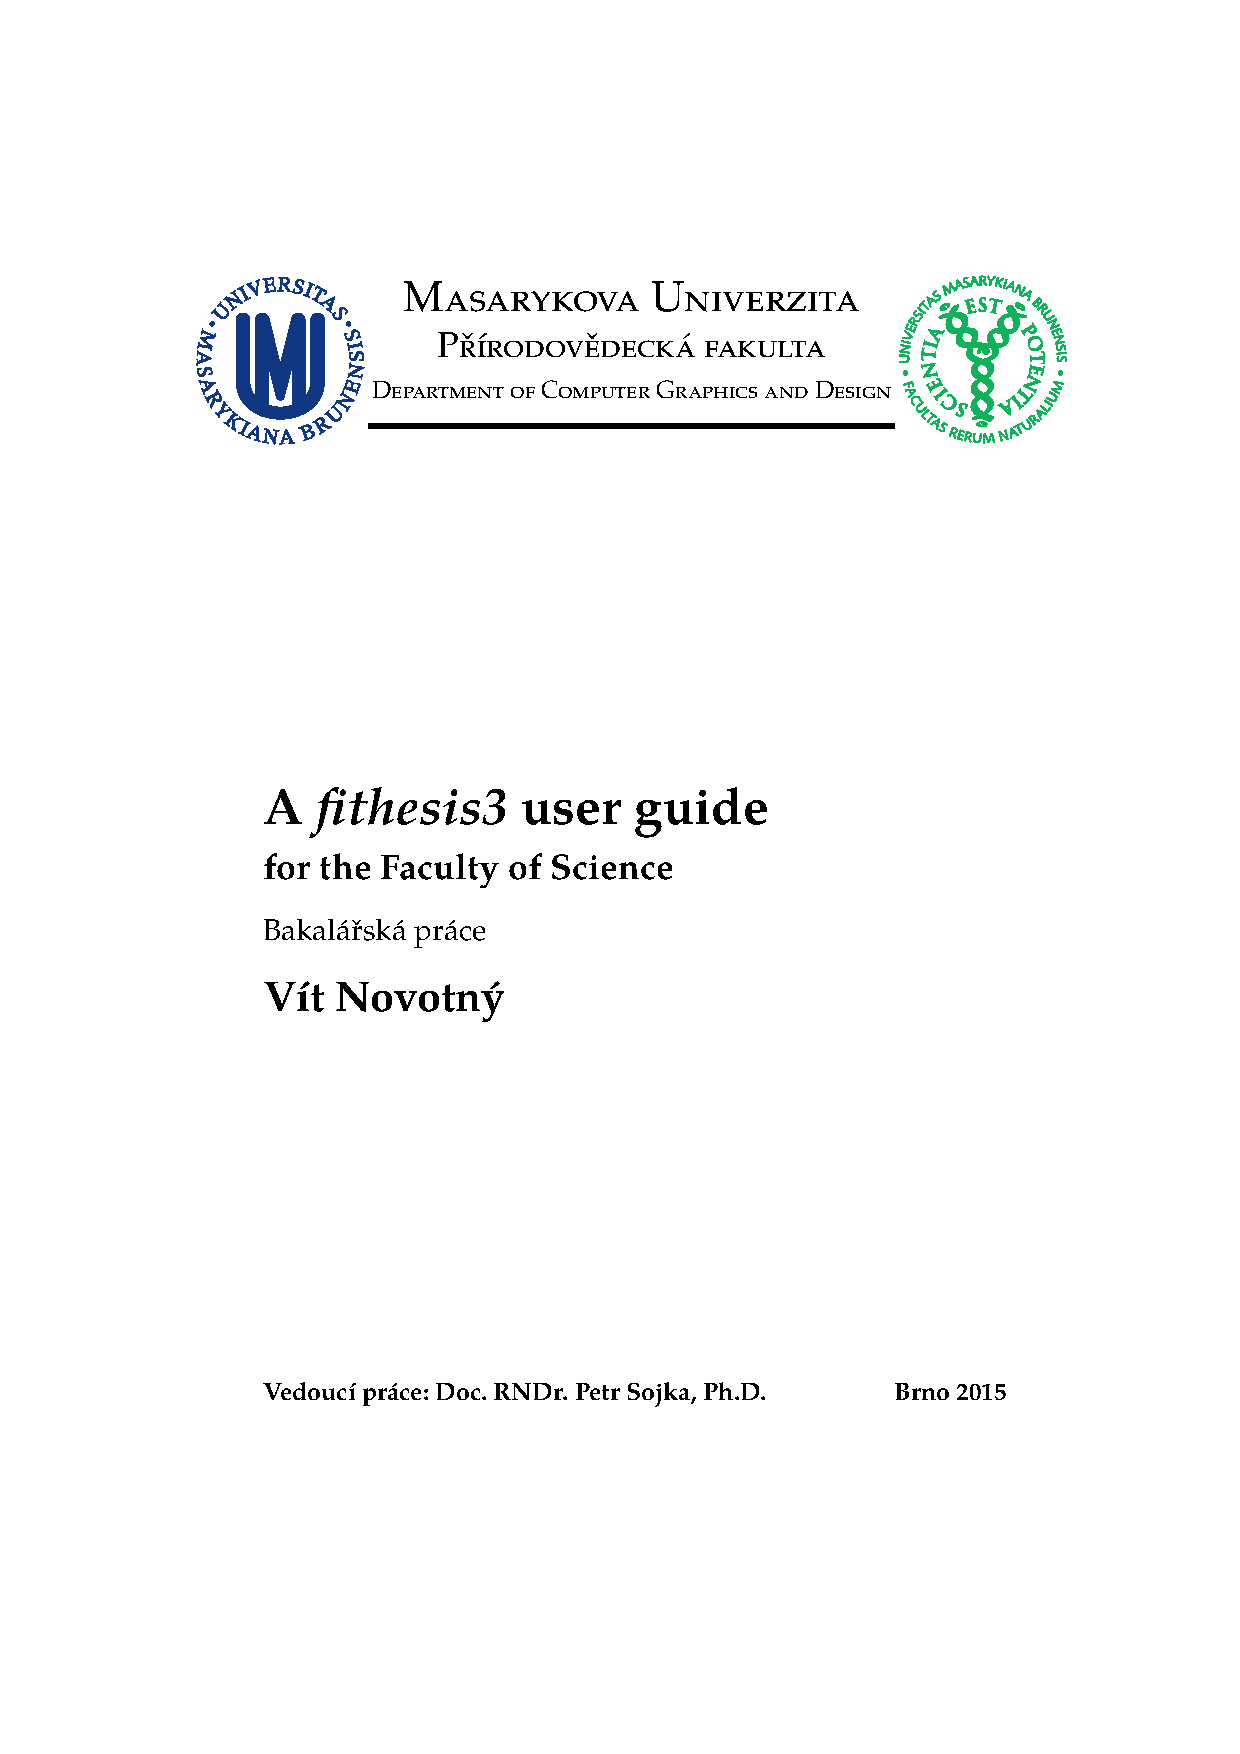
\includepdf[pages=-]{misc/sci.pdf}

\fakechapter{A \textsf{fithesis3} user guide for the Faculty of
  Economics and Administration}
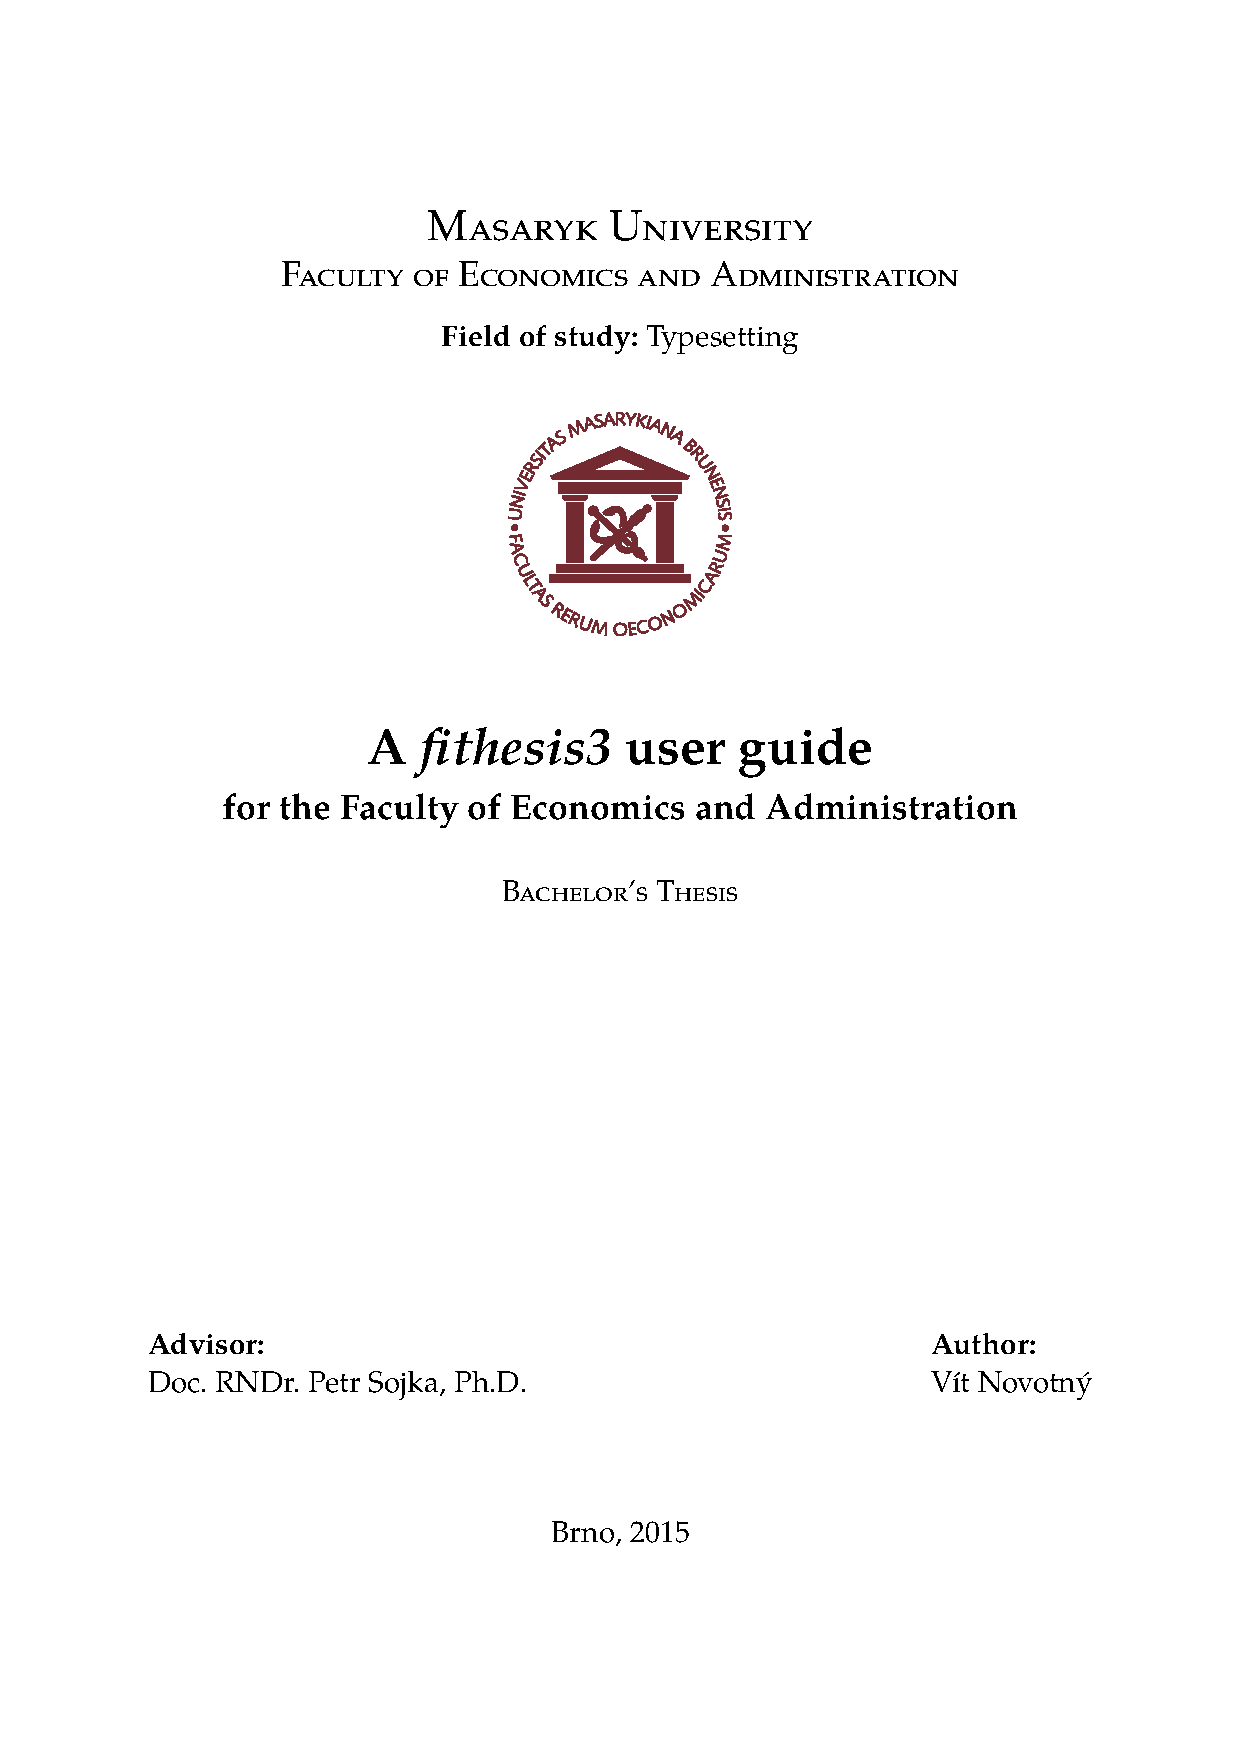
\includepdf[pages=-]{misc/econ.pdf}

\fakechapter{A \textsf{fithesis3} user guide for the Faculty of
  Social Studies}
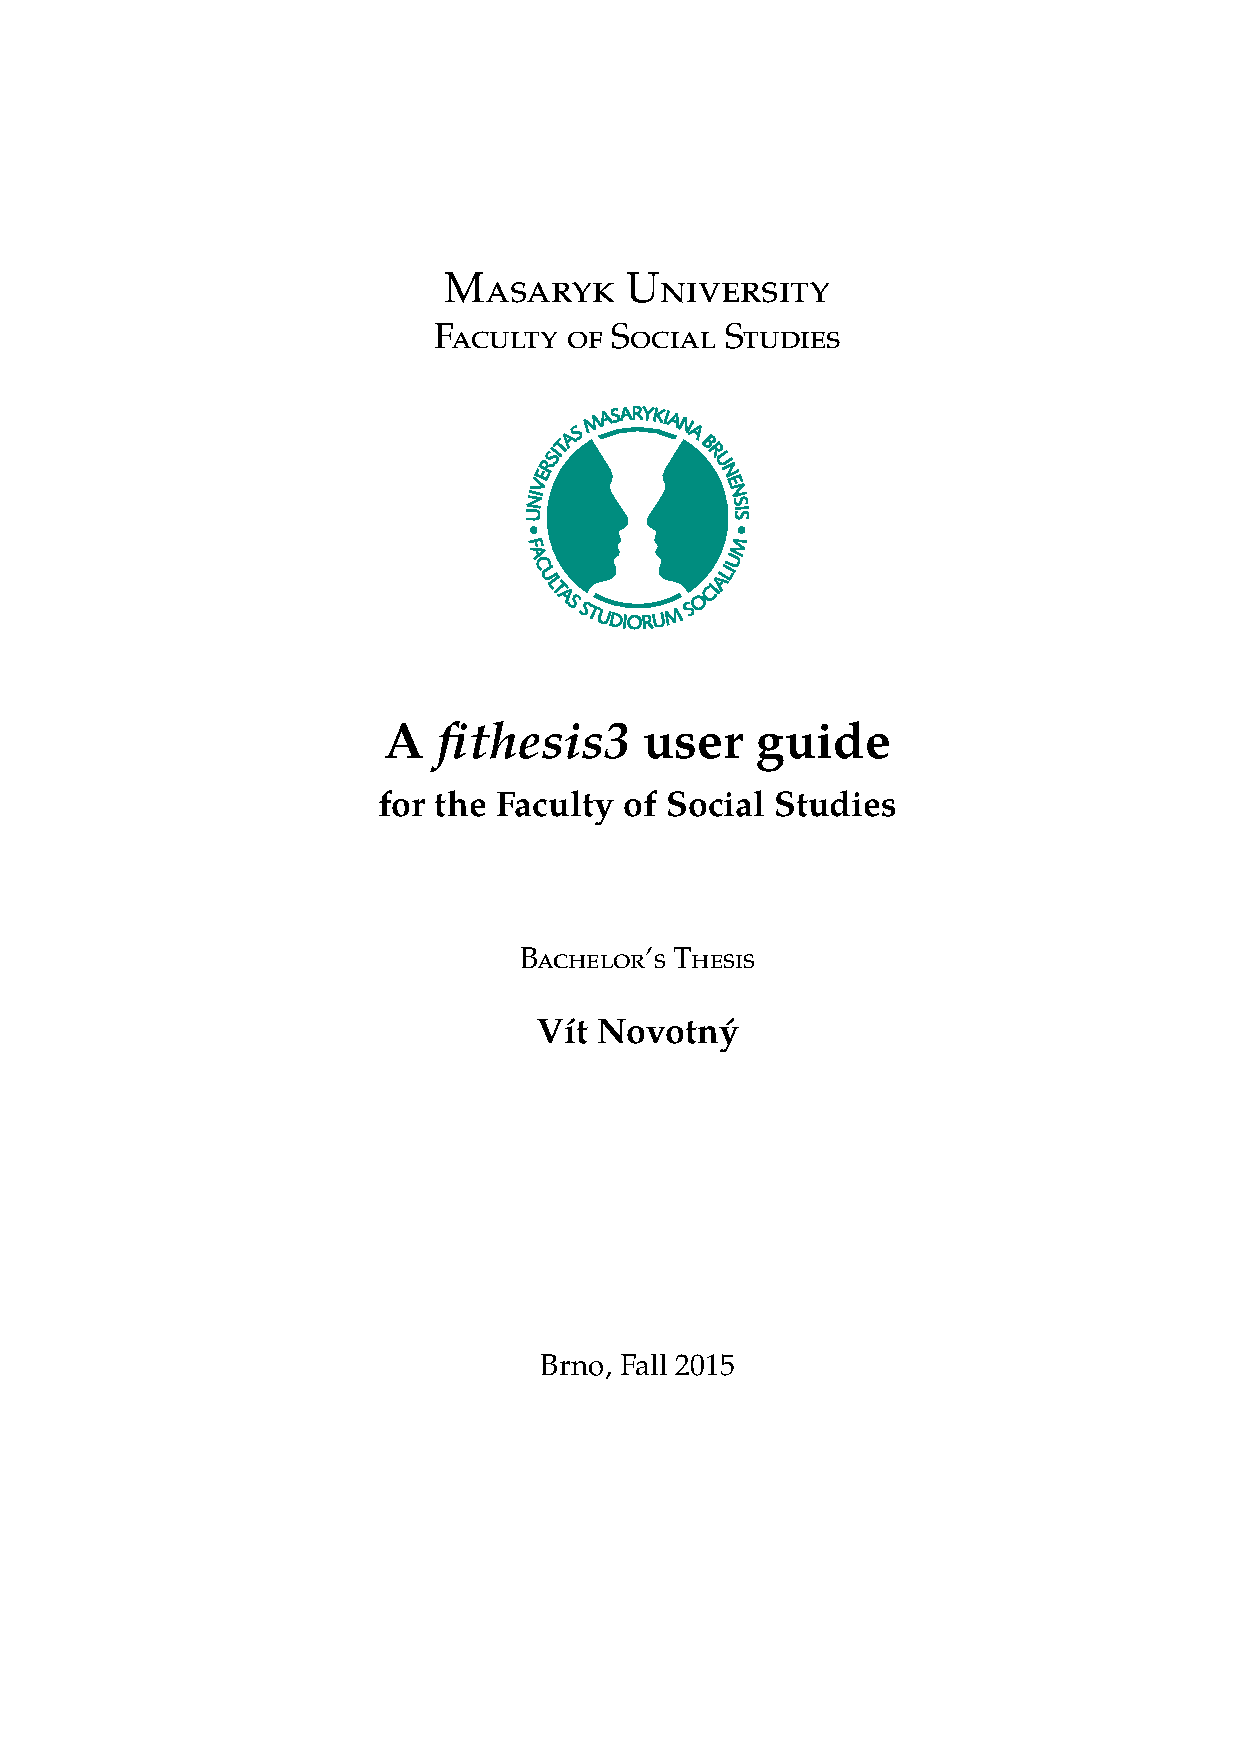
\includepdf[pages=-]{misc/fss.pdf}

\fakechapter{A \textsf{fithesis3} user guide for the Faculty of Law}
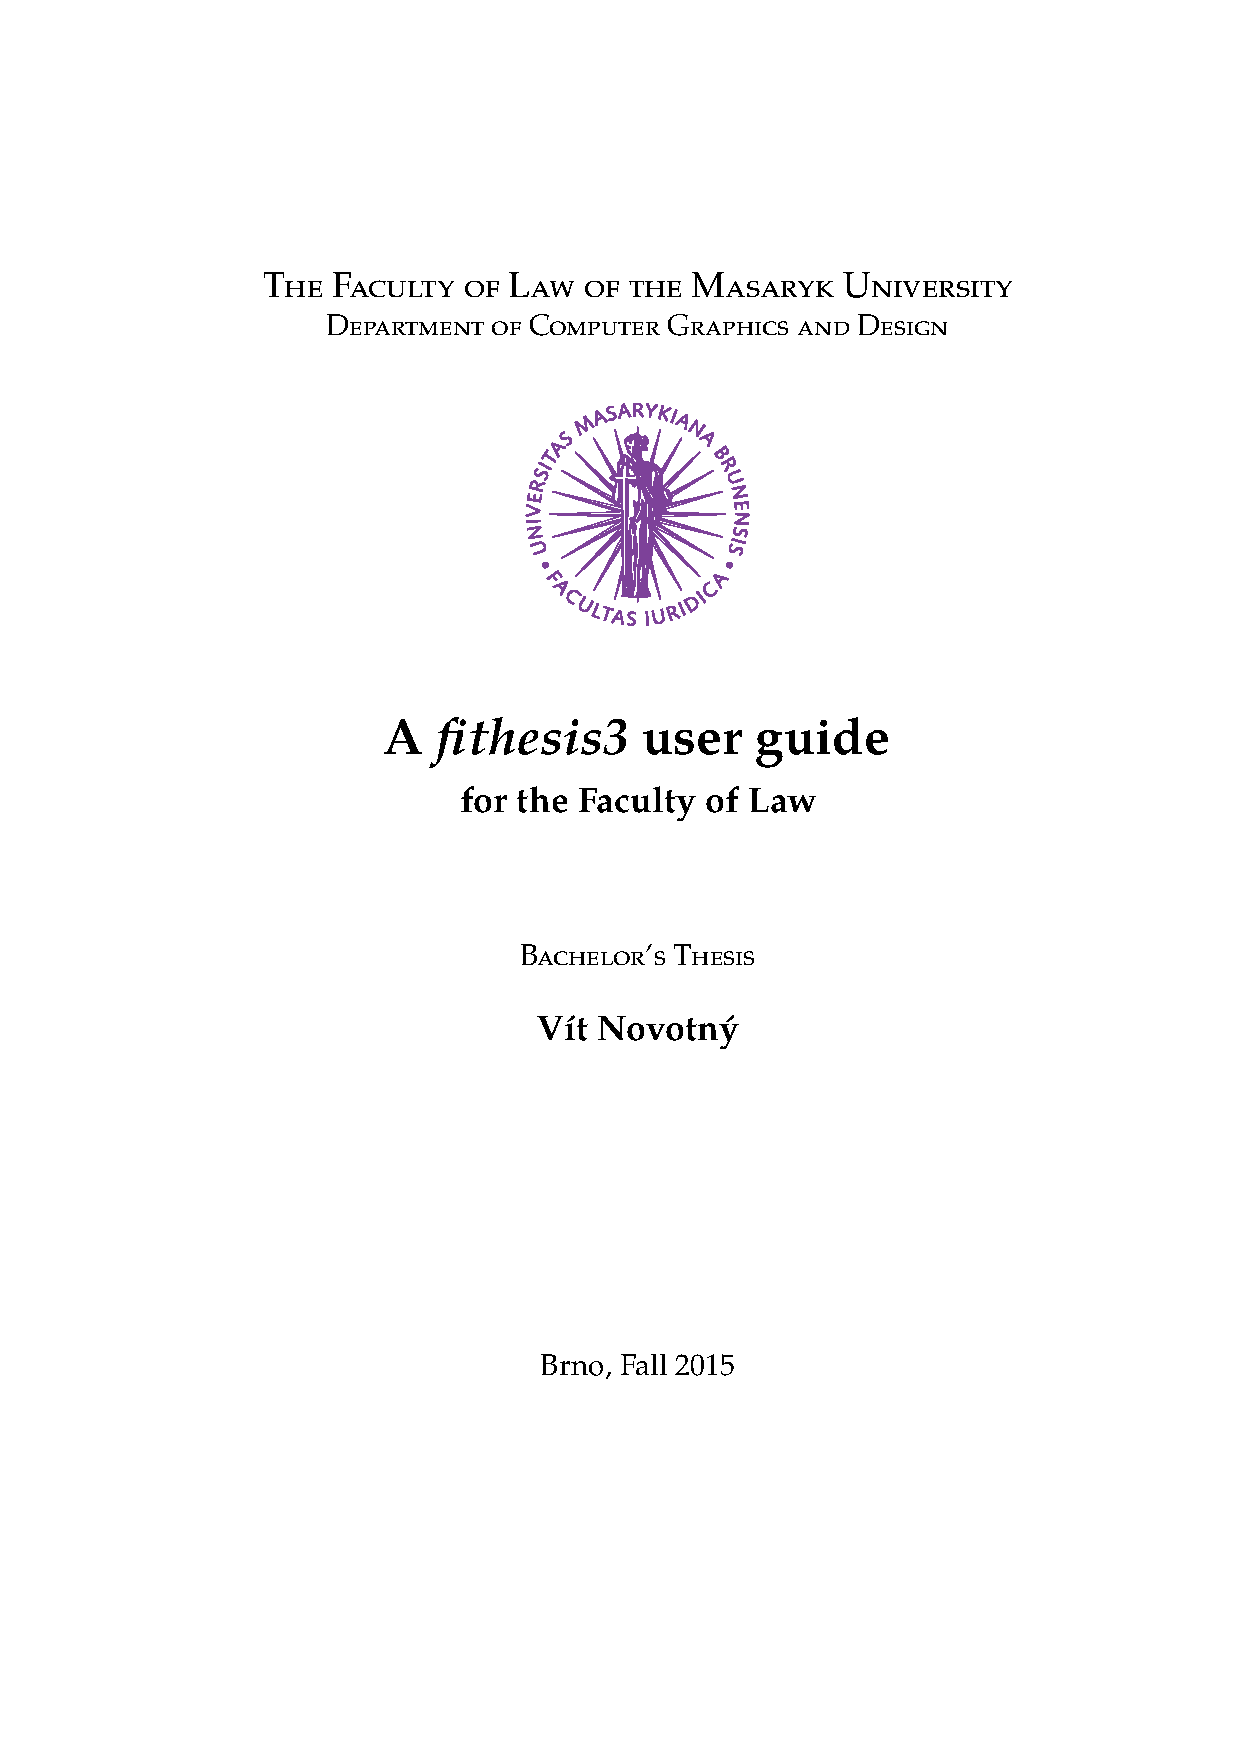
\includepdf[pages=-]{misc/law.pdf}

\fakechapter{A \textsf{fithesis3} user guide for the Faculty of
  Medicine}
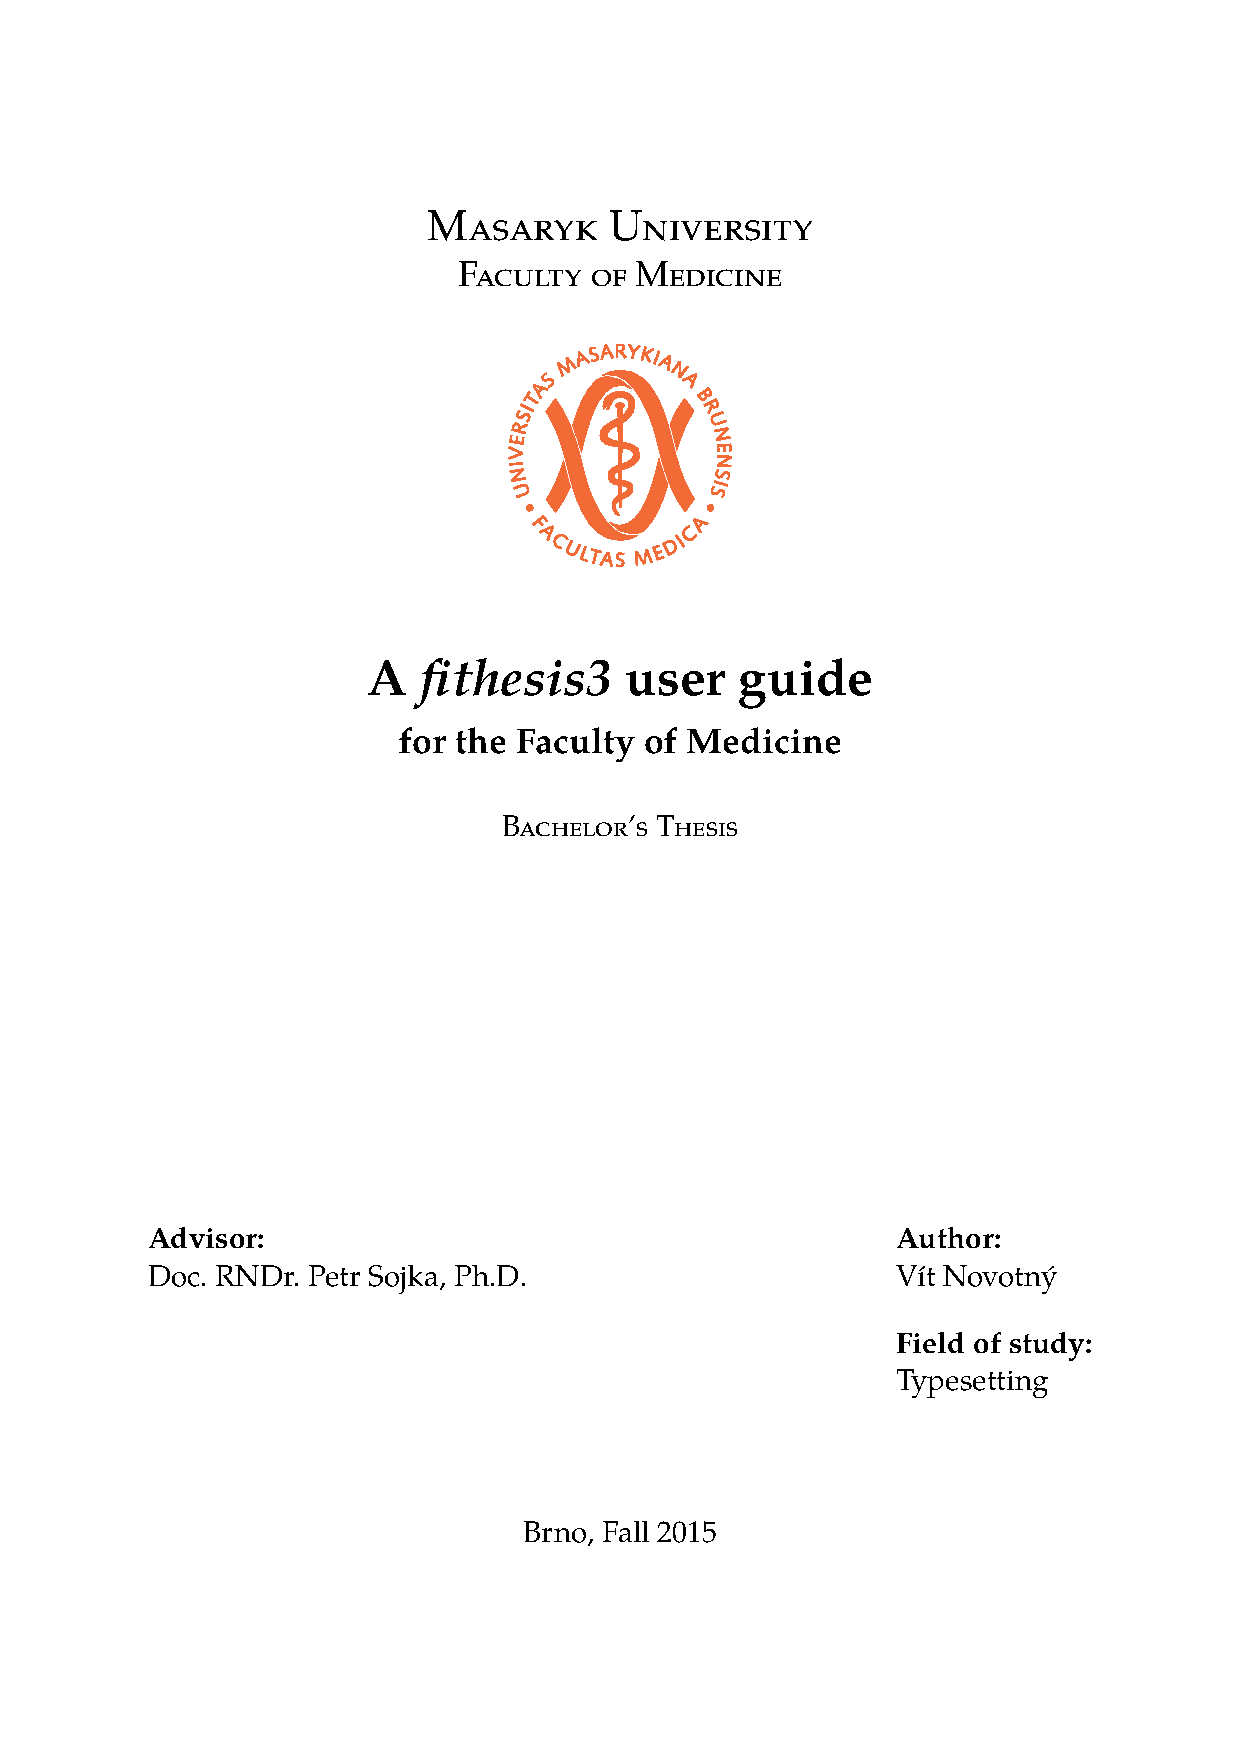
\includepdf[pages=-]{misc/med.pdf}

\fakechapter{A \textsf{fithesis3} user guide for the Faculty of
  Education}
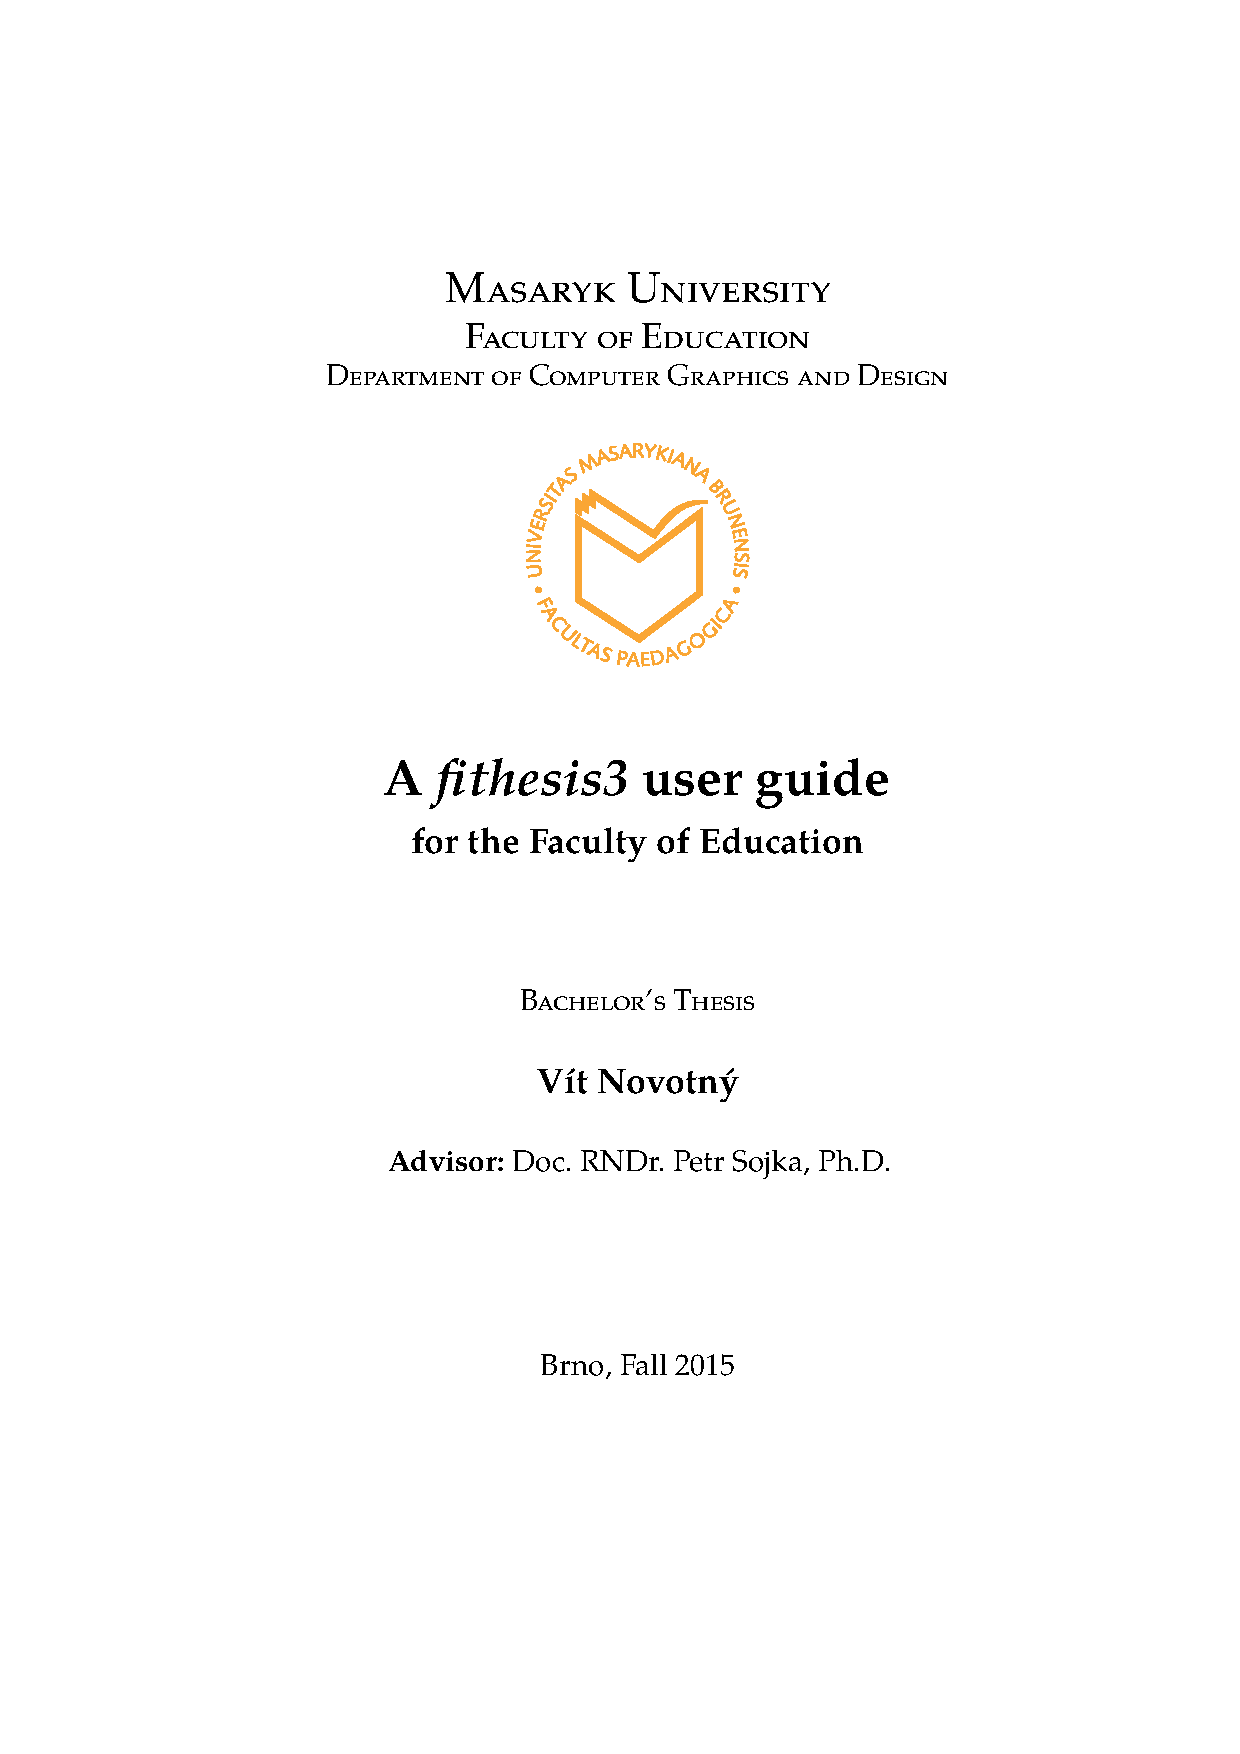
\includepdf[pages=-]{misc/ped.pdf}

\fakechapter{A \textsf{fithesis3} user guide for the Faculty of
  Arts}
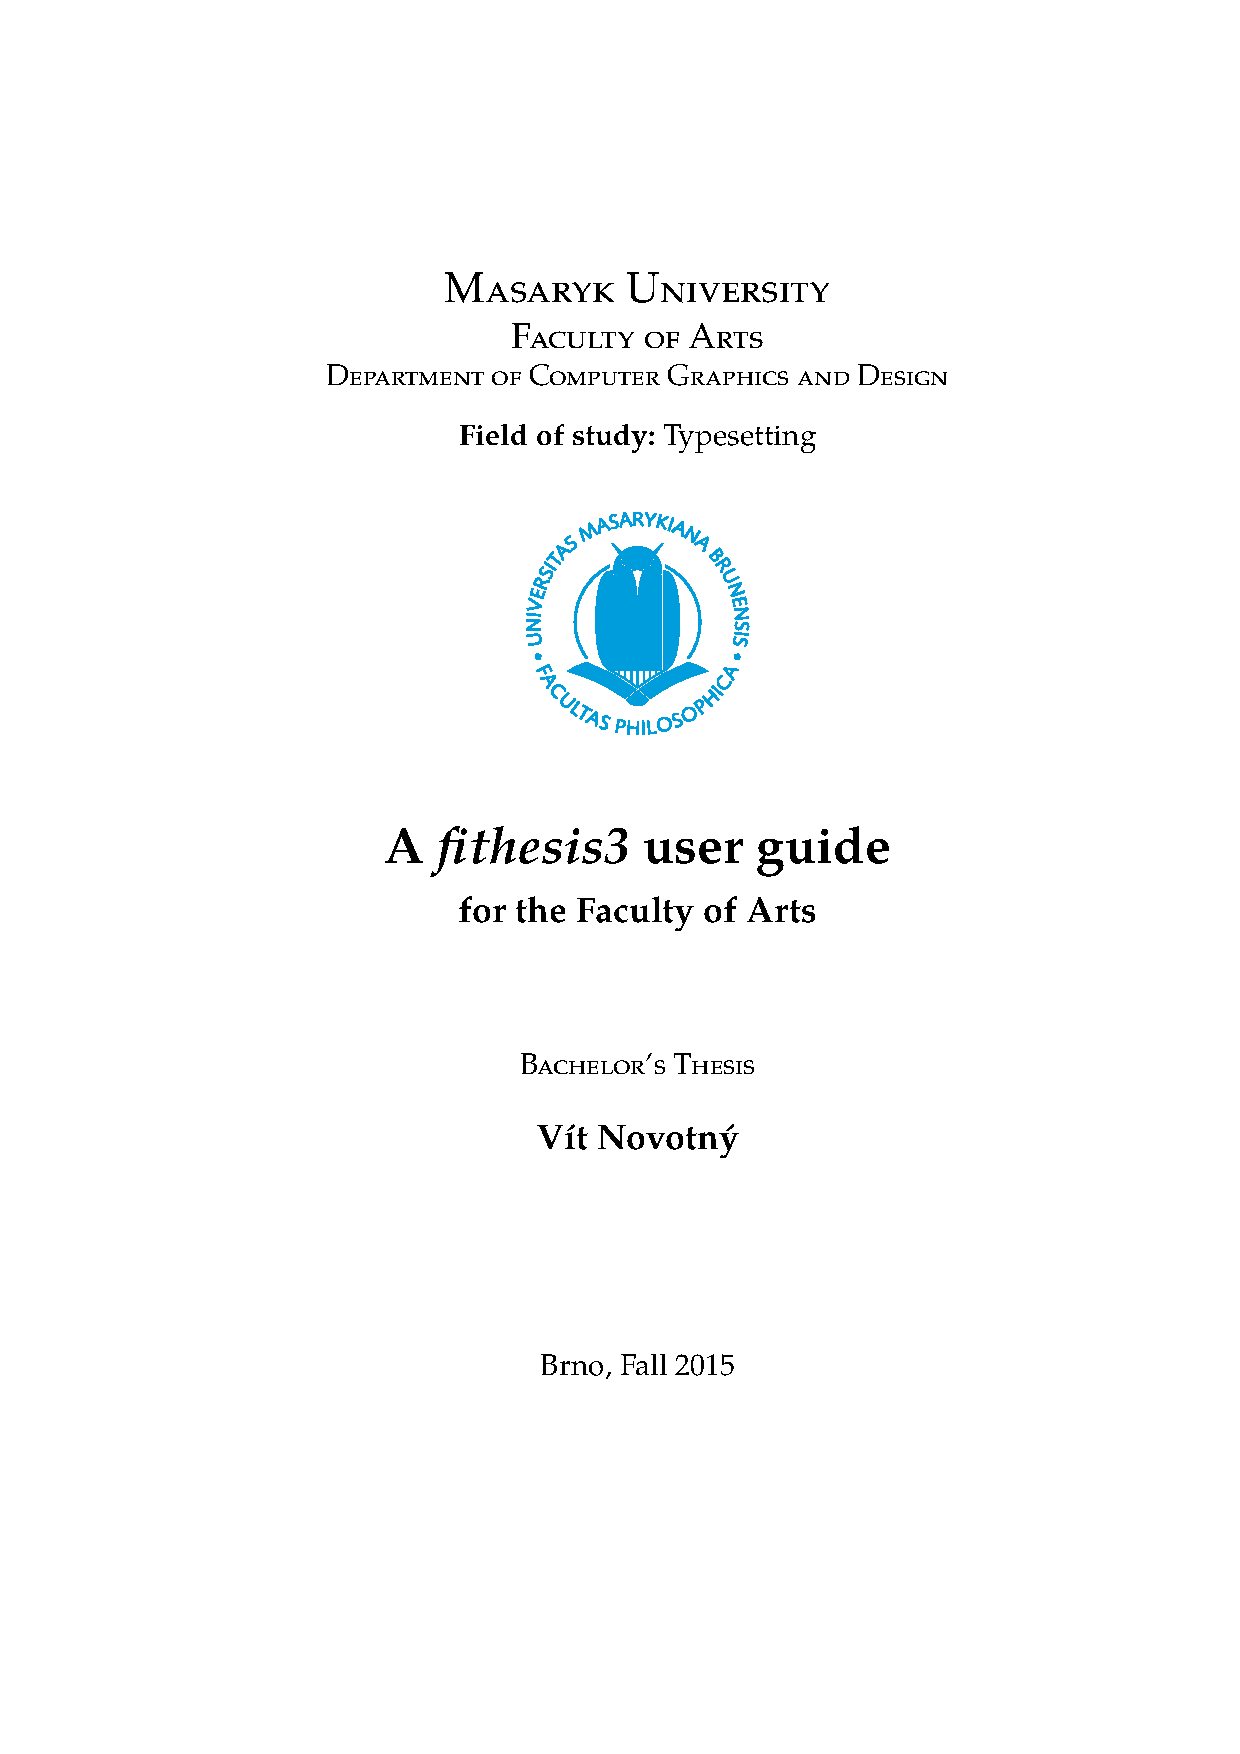
\includepdf[pages=-]{misc/phil.pdf}

\fakechapter{A \textsf{fithesis3} user guide for the Faculty of
  Sports Studies}\label{sec:fspsguide}
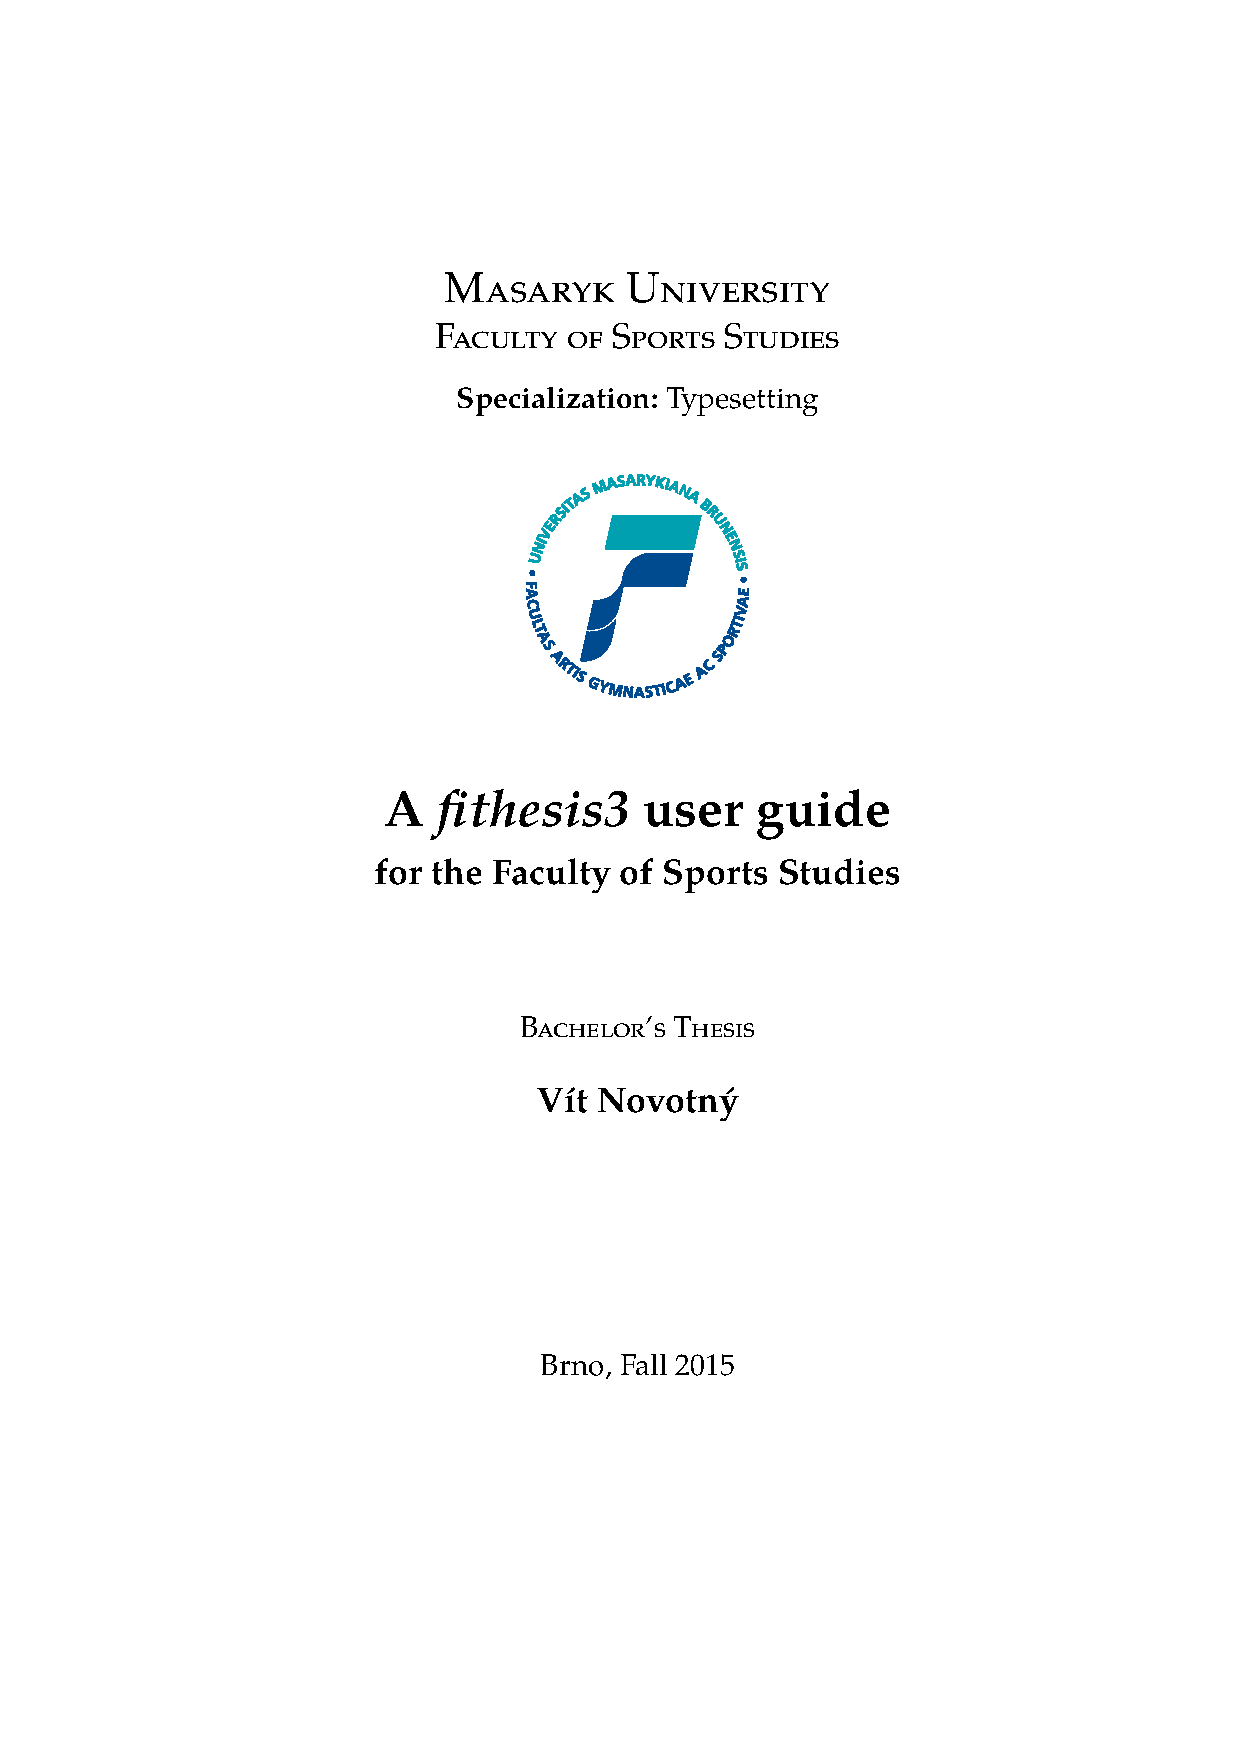
\includepdf[pages=-]{misc/fsps.pdf}

\fakechapter{The technical documentation of
  \textsf{fithesis3}}\label{sec:techdoc}
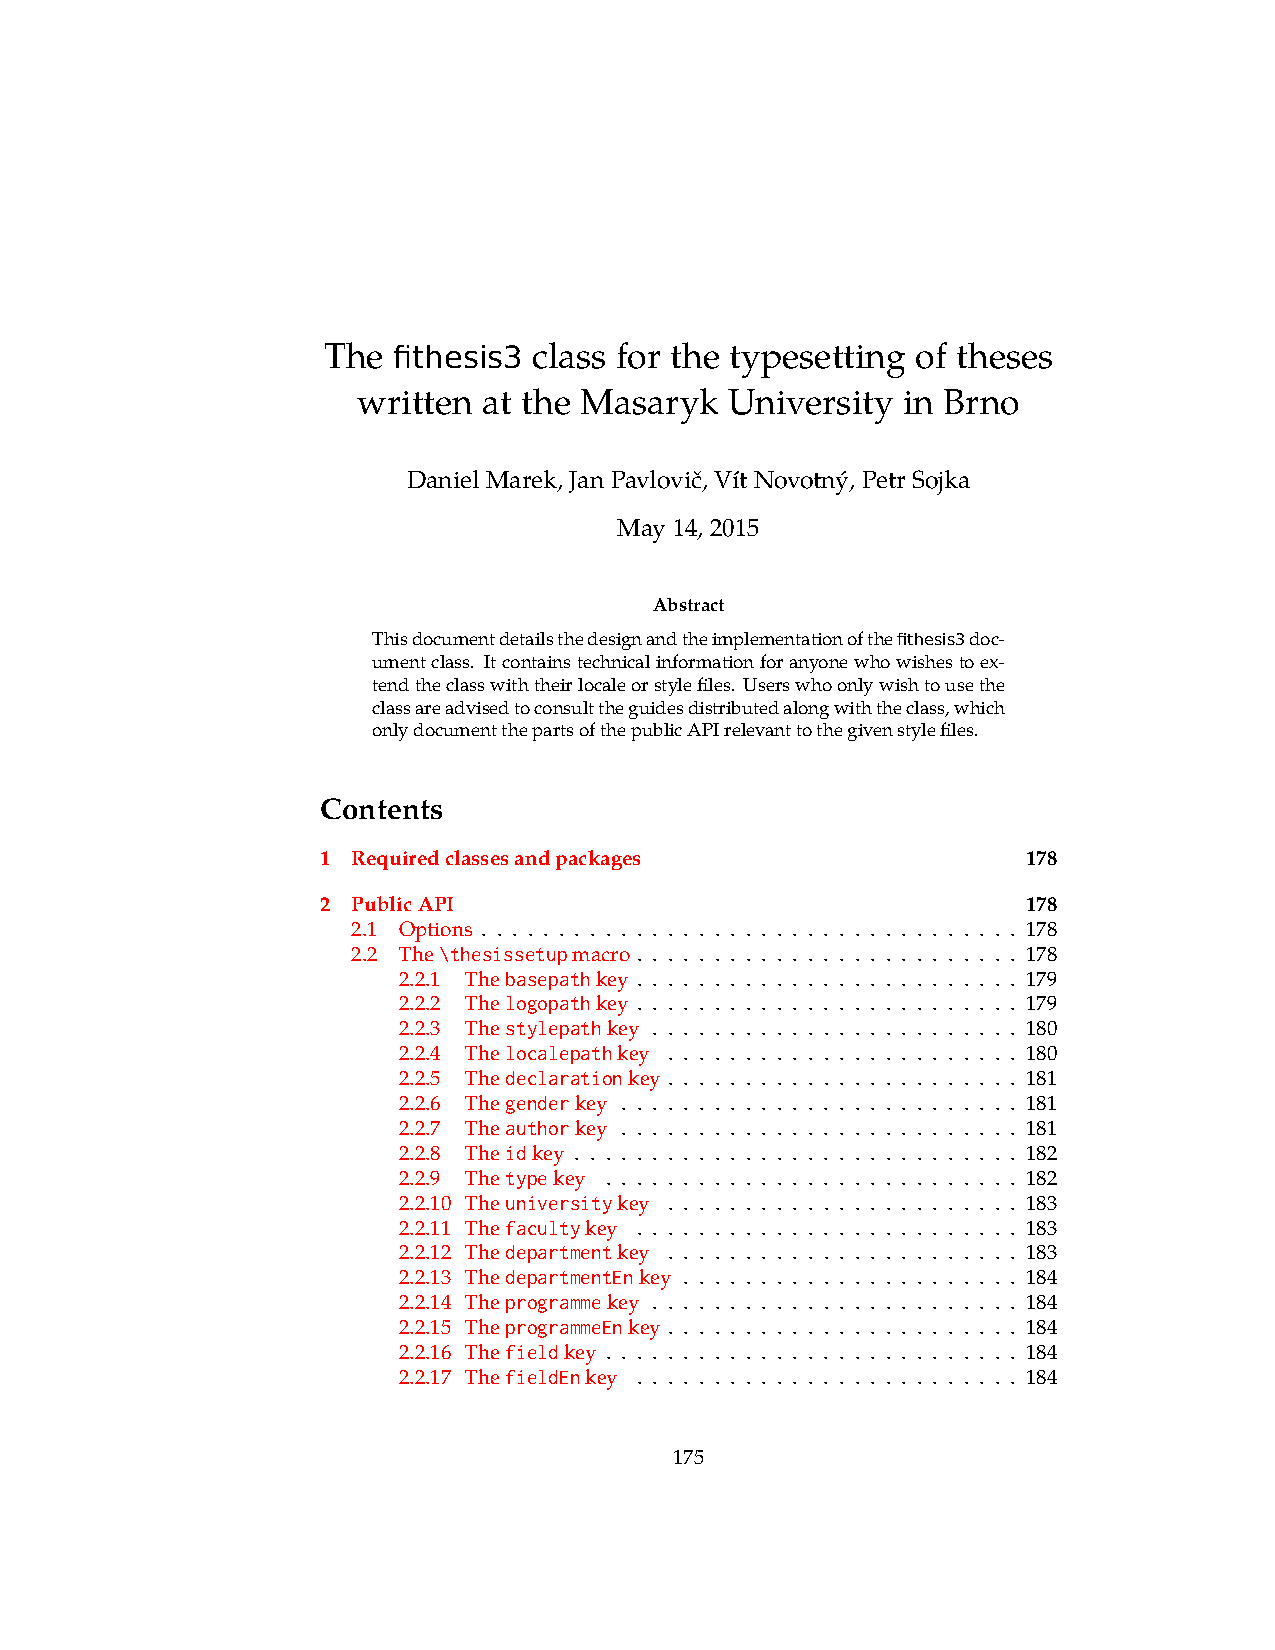
\includepdf[pages=-]{misc/fithesis.pdf}
\end{appendices}

% Bibliography
\newpage
%\nocite{*}
\tolerance=300
\emergencystretch=1em
\printbibliography[heading=bibintoc]
\par

% Glossary
\newpage
\printglossaries

% Index
\printindex
\end{document}
